\documentclass[11pt]{ctexart}
\usepackage[utf8]{inputenc}
\usepackage[left=1in,right=1in,top=1.2in,bottom=1.2in]{geometry}
\usepackage{fancyhdr}
\usepackage{amsmath}
\usepackage{amssymb}
\usepackage{multicol}
\usepackage{ctex}
\usepackage{hyperref}
\usepackage{listings}
\usepackage{xcolor}
\usepackage{graphicx,hyperref,url}
\usepackage{minted}
\usepackage{caption}
\usepackage{subfigure}
\usepackage{listings}
\usepackage{color}

\definecolor{dkgreen}{rgb}{0,0.6,0}
\definecolor{gray}{rgb}{0.5,0.5,0.5}
\definecolor{mauve}{rgb}{0.58,0,0.82}

\usepackage[T1]{fontenc}
\usepackage{mathpazo}
\usepackage{fontspec}
\setmainfont{TeX Gyre Pagella}
\setCJKmainfont[ItalicFont=Noto Sans CJK SC Bold, BoldFont=Noto Serif CJK SC Black]
{Noto Serif CJK SC}

\lstset{frame=tb,
  language=Python,
  aboveskip=3mm,
  belowskip=3mm,
  showstringspaces=false,
  columns=flexible,
  basicstyle={\small\ttfamily},
  numbers=none,
  numberstyle=\tiny\color{gray},
  keywordstyle=\color{blue},
  commentstyle=\color{dkgreen},
  stringstyle=\color{mauve},
  breaklines=true,
  breakatwhitespace=true,
  tabsize=3
}

% \usepackage{titlesec}
% \titlespacing\section{0pt}{15pt}{0pt}
% \titlespacing\subsection{0pt}{5pt}{0pt}
% \titlespacing\subsubsection{0pt}{5pt}{0pt}

\usepackage{enumitem}
\setlist{nolistsep}

\pagestyle{fancy}
\fancyhead[L]{East China Normal University}
\fancyhead[R]{\thepage}
\fancyfoot[C]{}

\fancypagestyle{plain}
{
\fancyhead[L]{East China Normal University}
\fancyhead[R]{\thepage}
\fancyfoot[C]{}
}

\ctexset{section/format=\Large\bfseries}



\setcounter{page}{1}

\title{华东师范大学软件工程实验报告}
\author{谢嘉东\ 10185101247\ \ 陈俊潼\ 10185101210}
\date{May 2020}

\begin{document}

\maketitle

\thispagestyle{empty}

\begin{itemize}
    \item 课程名称:数字图像处理
    \item 年级:2018 级本科
    \item 实验编号:实验 005
    \item 上机实践日期:2020.5
\end{itemize}

\tableofcontents

\thispagestyle{empty}

\newpage

\section{分工情况}

组内两人共同查阅资料,完善代码,完成了实验部分和附加题。

实验报告由两人共同撰写。

\section{实验目的}

\begin{itemize}
    \item [1] 了解 Python OpenCV 库对图像的基本操作
    \item [2] 使用 python 语言以及 cv 等图像处理库函数,实现图像恢复模块的实验。
    \item [3] 对图像的退化过程建立相应的数学模型,然后通过求解该逆问题获得图像的恢复模型并对原始图像进行合理估计。
\end{itemize}

\section{实验内容}

图像增强旨在改善图像质量。而图像恢复力求保持图像的本来面目,以保真原则为前提,找出图像降质的原因,描述其物理过程,提出数学模型。恢复的过程是沿着降质的逆过程来重现原始图像。

图像恢复是图像处理中的一个重要问题,对于改善图像质量具有重要的意义。解决该问题的关键是对图像的退化过程建立相应的数学模型,然后通过求解该逆问题获得图像的恢复模型并对原始图像进行合理估计。

图像退化即图像质量降质。图像退化的典型表现是图像出现模糊、失真,出现附加噪声等。由于图像的退化,在图像接受端显示的图像已不再是传输的原始图像,图像效果明显变差。

\subsection*{退化函数的估计}

在图像复原中,我们需要对退化函数进行估计。主要有观察法,实验法,数学建模法。

观察法通过选择噪声较小的子图像(减少噪声的影响)来得到 $H(u,v)$ ,然后根据此信息来构建全图的 $H(u,v)$ ,之后利用后面的复原方法来复原。

实验法是指我们可以使用或设计一个与图像退化过程相似的装置(过程),使其成像一个脉冲,可得到退化系统的冲激响应 $H(u,v) = \frac{G(u,v)}{A}$。

而建模估计则是从引起图像退化的基本原理进行推导,进而对原始图像进行模拟,在模拟过程中调整模型参数以获得尽可能精确的退化模型。课本中有两种模型,大气湍流模型和运动模糊模型。

\subsection*{图像恢复}

图像复原算法有线性和非线性两类。

线性算法通过对图像进行逆滤波来实现反卷积,这类方法方便快捷,无需循环或迭代,直接可以得到反卷积结果,然而,它有一些局限性,比如无法保证图像的非负性。

而非线性方法通过连续的迭代过程不断提高复原质量,直到满足预先设定的终止条件,结果往往令人满意。但是迭代程序导致计算量很大,图像复原时耗较长,有时甚至需要几个小时。所以实际应用中还需要对两种处理方法综合考虑,进行选择。

\section{实验原理}

利用 numpy 、matplotlib.pyplot 、cv2 、imageio 、skimage 以及 Pillow 中的 PIL 包来辅助完成实验。其中主要用到了:

\begin{itemize}
    \item cv.erode(src, dst, element=None, iterations=1) 
    \begin{itemize}
        \item src – input image; the number of channels can be arbitrary, but the depth should be one of CV\_8U, CV\_16U, CV\_16S, CV\_32F` or ``CV\_64F.
        \item dst – output image of the same size and type as src.
        \item element – structuring element used for erosion; if element=Mat() , a 3 x 3 rectangular structuring element is used.
        \item anchor – position of the anchor within the element; default value (-1, -1) means that the anchor is at the element center.
        \item iterations – number of times erosion is applied.
        \item borderType – pixel extrapolation method
        \item borderValue – border value in case of a constant border
    \end{itemize}
\end{itemize}
    
    
\begin{itemize}
    \item cv.dilate(src, dst, element=None, iterations=1)
     \begin{itemize}
    \item src – input image; the number of channels can be arbitrary, but the \item depth should be one of CV\_8U, CV\_16U, CV\_16S, CV\_32F` or ``CV\_64F.
    \item dst – output image of the same size and type as src.
    \item element – structuring element used for dilation; if element=Mat() , a 3 x 3 rectangular structuring element is used.
    \item anchor – position of the anchor within the element; default value (-1, -1) means that the anchor is at the element center.
    \item iterations – number of times dilation is applied.
    \item borderType – pixel extrapolation method
    \item borderValue – border value in case of a constant border
    \end{itemize}
\end{itemize}
   
    
    
    \begin{itemize}
        \item
          \texttt{cv.GetRotationMatrix2D}(center, angle, scale, mapMatrix)
          \begin{itemize}
          \item
            \textbf{center} -- Center of the rotation in the source image.
          \item
            \textbf{angle} -- Rotation angle in degrees. Positive values mean
            counter-clockwise rotation (the coordinate origin is assumed to be
            the top-left corner).
          \item
            \textbf{scale} -- Isotropic scale factor.
          \item
            \textbf{map\_matrix} -- The output affine transformation, 2x3
            floating-point matrix.
          \end{itemize}
    \end{itemize}
    
    
    \begin{itemize}
    \item
      \texttt{cv.WarpAffine}(src, dst, mapMatrix,
      flags=CV\emph{INTER}LINEAR+CV\emph{WARP}FILL\_OUTLIERS, fillval=(0, 0,
      0, 0))
      \begin{itemize}
      \item
        \textbf{src} -- input image.
      \item
        \textbf{dst} -- output image that has the size \texttt{dsize} and
        the same type as \texttt{src} .
      \item
        \textbf{M} -- \(2 \times 3\) transformation matrix.
      \item
        \textbf{dsize} -- size of the output image.
      \item
        \textbf{flags} -- combination of interpolation methods
      \item
        \textbf{borderMode} -- pixel extrapolation method
      \item
        \textbf{borderValue} -- value used in case of a constant border; by
        default, it is 0.
        \end{itemize}  
    \end{itemize}

    \begin{itemize}
    \item numpy.array(object, dtype=None, copy=True, order='K', subok=False, ndmin=0)
    \begin{itemize}
        \item object : array\_like
        \item dtype : data-type, optional
        \item copy : bool, optional
        \item order : {‘K’, ‘A’, ‘C’, ‘F’}, optional
        \item subok : bool, optional
        \item ndmin : int, optional
    \end{itemize}

    \item scipy.ndimage.filters.gaussian\_filter(input, sigma, order=0, output=None, mode='reflect', cval=0.0, truncate=4.0)
    \begin{itemize}
        \item input : array\_like, Input array to filter.
        \item sigma : scalar or sequence of scalars
    \end{itemize}
   
   
   \item scipy.ndimage.filters.minimum\_filter(input, sigma, order=0, output=None, mode='reflect', cval=0.0, truncate=4.0)
    \begin{itemize}
        \item input : array\_like, Input array to filter.
        \item sigma : scalar or sequence of scalars
    \end{itemize}

\item scipy.ndimage.filters.maximum\_filter(input, sigma, order=0, output=None, mode='reflect', cval=0.0, truncate=4.0)
    \begin{itemize}
        \item input : array\_like, Input array to filter.
        \item sigma : scalar or sequence of scalars
    \end{itemize}
\end{itemize}

\section{实验方法}

\subsection{退化函数的估计}

\subsubsection{大气湍流模型}

大气湍流模型通用形式为 $H(u,v)=e^{-k(u^2+v^2)^{\frac{5}{6}}}$ 。

在实现该滤波器的过程中,由于需要中心化,所以要注意 $u,v$ 应该分别替换为各自与频率中心之差(i.e.假设频率中心为 $(\frac{M}{2},\frac{N}{2})$ ,则替换为 $u-\frac{M}{2}$ 和 $v-\frac{N}{2}$ )。其傅里叶频谱图如下:

\begin{figure}[htbp]
    \centering
    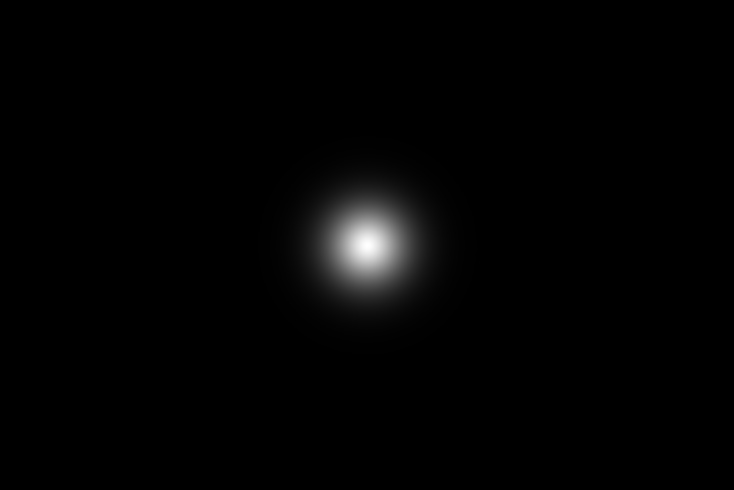
\includegraphics[width=0.6\textwidth]{output/turbulence_H.jpg}
\end{figure}

我们在实验过程中,通过对不同参数下的效果调整发现, $k$ 是与湍流性质有关的常数(i.e. $k$ 越大,图像越模糊,与高斯低通滤波器有着相同的形式)。

\subsubsection{运动模糊模型}

运动模糊是景物图象中的移动效果。它比较明显地出现在长时间暴光或场景内的物体快速移动的情形里。

运动模糊模型退化函数为: $H(u,v)=\frac{Tsin[\pi (ua+vb)])}{\pi (ua+vb)}e^{-j\pi (ua+vb)}$ 。

其中 $T$ 表示曝光时间, $a$ 和 $b$ 分别表示水平和垂直方向上的移动量。

和大气湍流类似的,在实现该滤波器的过程中,由于需要中心化,所以要注意 $u,v$ 应该分别替换为各自与频率中心之差(i.e.假设频率中心为 $(\frac{M}{2},\frac{N}{2})$ ,则替换为 $u-\frac{M}{2}$ 和 $v-\frac{N}{2}$ )。

\subsection{图像恢复}

\subsubsection{直接逆滤波}

由退化函数 $H$ 退化的图像复原的最简单的方法是直接做逆滤波,设图像退化前的傅里叶变换为 $F(u,v)$ ,退化后的傅里叶变换为 $G(u,v)$ ,系统函数即退化函数的傅里叶变换为 $H(u,v)$ 。

所谓直接逆滤波,就是用退化函数除退化图像的傅里叶变换,得到退化前图像的傅里叶变换的估计,$\hat{F}(u,v)$ 为 $F(u,v)$ 的估计,则 $\hat{F}(u,v)=\frac{G(u,v)}{H(u,v)}$ ,同时 $G(u,v)=F(u,v)H(u,v)+N(u,v)$ ,其中 $N(u,v)$ 为噪声的傅里叶变换。

因此,可得 $\hat{F}(u,v)=F(u,v)+\frac{N(u,v)}{H(u,v)}$ ,于是可知,即使知道退化函数,也不能准确的复原图像,因为 $N(u,v)$ 是未知,甚至有更糟的情况是如果退化函数是零或是非常小的值,则 $\frac{N(u,v)}{H(u,v)}$ 的值比较大,很容易支配 $F(u,v)$ 的估计值。

解决这个问题的一种方法是限制滤波的频率,从频谱图可知,高频分量的值接近 $0$ ,而 $H(0,0)$ 在频率域中通常是 $H(u,v)$ 的最高值。因此可缩短滤波半径,使通过的频率接近原点,减少遇到零值的概率。

而在本实验中,我们经过多次参数的调整均无法取得比较理想的效果。于是我们通过在利用相同参数的方式进行运动模糊以及对其进行直接逆滤波来得到了较好的效果。

\subsubsection{维纳滤波}

维纳滤波器提出的一种以最小平方为最优准则的线性滤波器。在一定的约束条件下,其输出与一给定函数(通常称为期望输出)的差的平方达到最小,通过数学运算最终可变为一个托布利兹方程的求解问题。

假设维纳滤波器的输入信号是 $s(t)$ 叠加噪声 $n(t)$。输出信号 $x(t)$ 通过滤波器 $g(t)$ 使用下面的卷积运算得到: $ x(t)=g(t)\times (s(t)+n(t))$

其中,$s(t)$ 是需要估计的原始信号,$n(t)$ 是噪声,$x(t)$ 是估计出的信号(我们希望它能等同于 $ s(t)$), $g(t)$ 是维纳滤波器 。

为了获得维纳滤波系数,考虑将信号 $w[n]$ 输入到一个 $N$ 阶维纳滤波器,系数 $a_{i}$ , $i\,=\,0,\,\ldots ,\,N$ ,$N$ 的滤波器的输出被记作 $x[n]$ ,这是由下式给出 $ x[n]=\sum _{i=0}^{N}a_{i}w[n-i]$ 。剩余误差来表示 $e[n]$ 的,被定义为 $e[n] = x[n] − s[n]$ 。

    \begin{figure}[htbp]
        \centering
        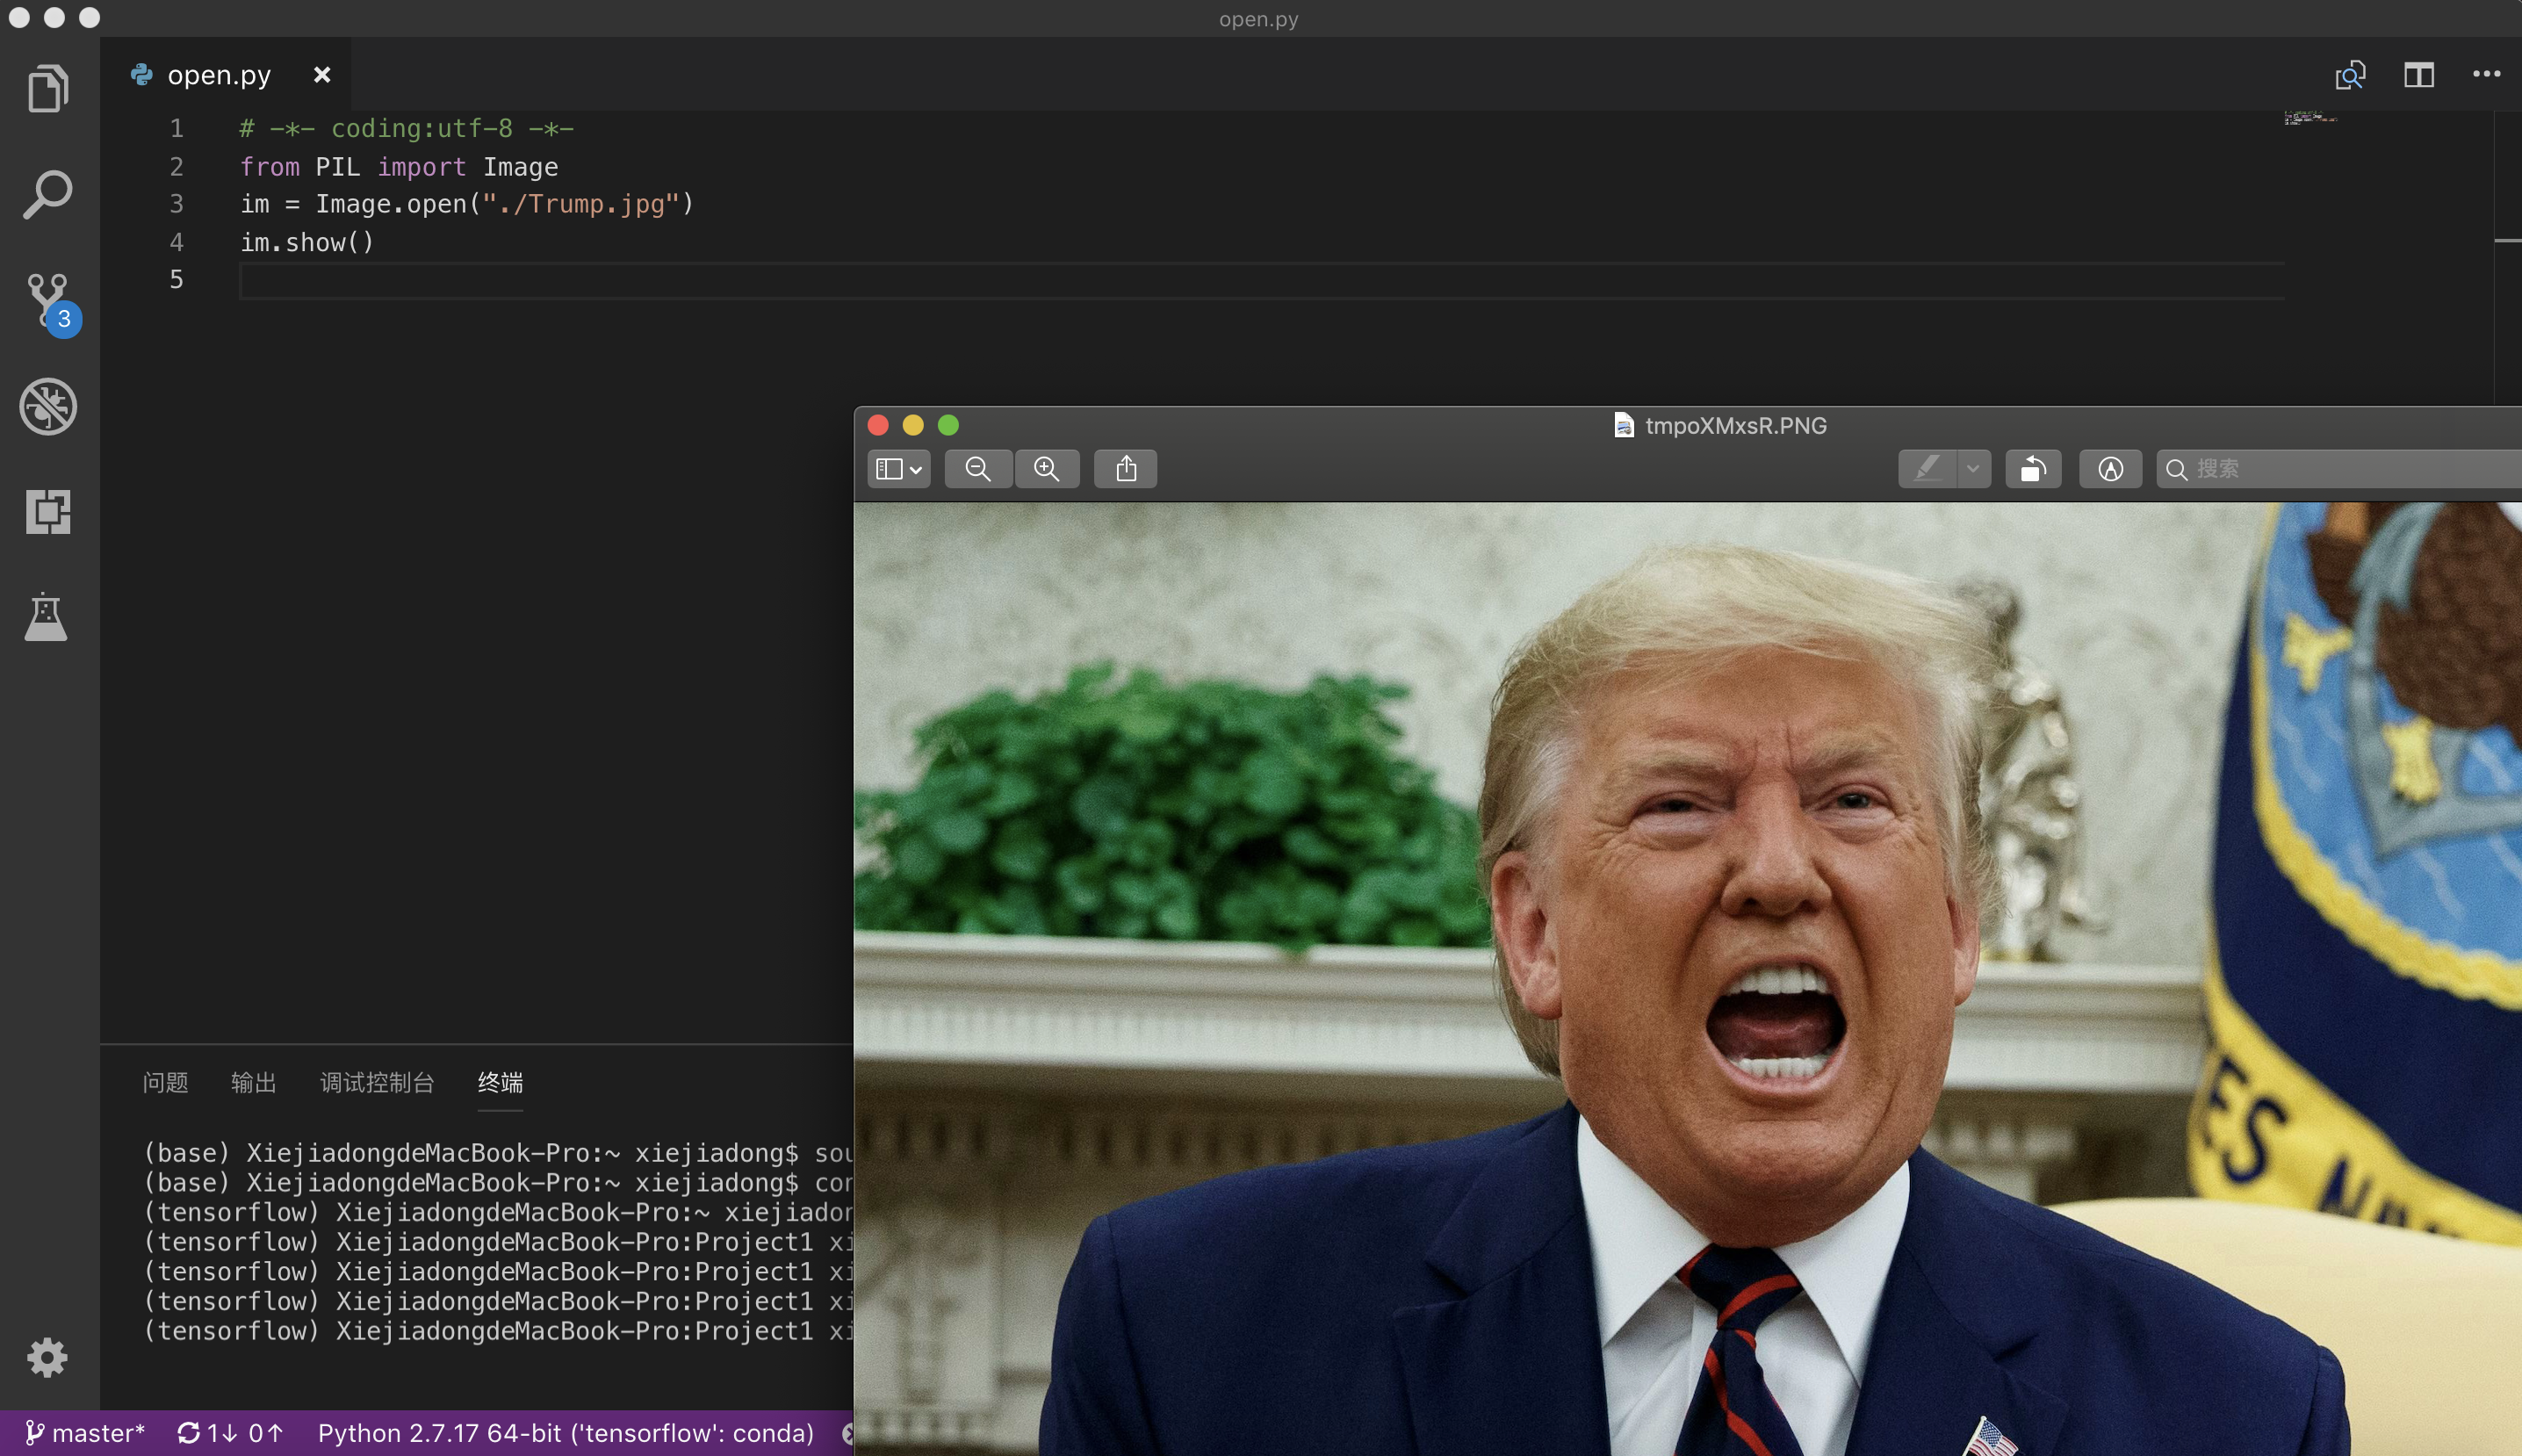
\includegraphics[width=0.6\textwidth]{./pic1.png}
  \end{figure}
  
同样的,我们为了获得较好的实验效果,通过在利用相同参数的方式进行运动模糊以及对其进行直接维纳滤波来得到了较好的效果。

\subsubsection{约束最小二乘方滤波器}

图像的退化过程可以表示为 $g(x,y)=H[f(x,y)]+\eta(x,y)$,表达为向量-矩阵形式为$g=Hf+\eta$。使用约束最小二乘法可以解决直接逆滤波方法对噪声敏感的问题。为了解决噪声敏感的问题,需将复原的最优化性建立在平滑度量上。因此,约束最小二乘法滤波使用了一个标准函数 C 和约束函数,定义如下:

$$
C = \sum_{x=0}^{M-1}\sum_{y=0}^{N-1}[\nabla^2f(x,y)]
$$

其约束为

$$
\parallel g-H\hat{f}\parallel^2 = \parallel \eta \parallel ^2
$$

其中,$\nabla^2$ 为拉普拉斯算子:

$$
\nabla^2 = 
\begin{bmatrix}
0 & -1 & 0 \\
-1 & 4 & -1 \\
0 & -1 & 0
\end{bmatrix}
$$

在频率域中,上述的约束函数 C 可以表示为 $C = \parallel P \hat{f} \parallel_2^2$,P 是拉普拉斯算子 $\nabla^2$ 的傅里叶变换。于是根据约束函数和约束条件可以建立拉格朗日函数:

$$
L(\hat{F}, \lambda) = \parallel P\hat{F} \parallel_2^2 + \lambda( 
\parallel G-H\hat{F}\parallel^2 - \parallel N \parallel ^2
)
$$

其中 $N$ 为加性噪声 $\eta$ 的傅里叶变换。在拉格朗日函数中对 $\hat{F}$ 求导,得到 $\hat{F}$ 的最小值为:

$$
\hat{F} (u,v) = \Big[\frac{H*(u,v)}{|H(u,v)| ^ 2 + \gamma|P(u,v)|^2}\Big] G(u,v)
$$

其中 $H*(u, v)$ 是 $H$ 的共轭函数。使用该式即可对图像进行复原操作。

\section{实验结果及分析}

基本完成了实验预期所要达到的要求。

最终的实验结果如下:

\subsection*{退化函数的估计}

\subsubsection*{大气湍流模型}

    \begin{figure}[htbp]
        \centering
        \subfigure[原图]{
            \begin{minipage}[t]{0.35\linewidth}
            \centering
            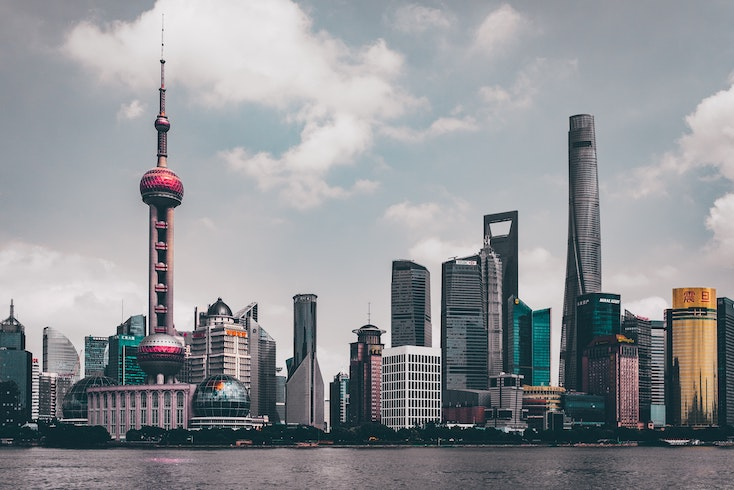
\includegraphics[width=0.9\textwidth]{input/1.1.jpg}
        \end{minipage}
        }
        \subfigure[k = 0.001]{
            \begin{minipage}[t]{0.35\linewidth}
            \centering
            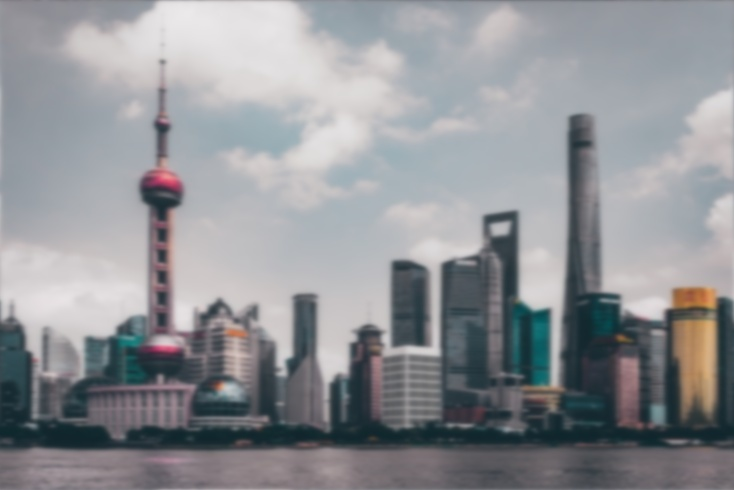
\includegraphics[width=0.9\textwidth]{output/1.1_turbulence_0.001.jpg}
            \end{minipage}
        }
                \subfigure[k = 0.0025]{
            \begin{minipage}[t]{0.35\linewidth}
            \centering
            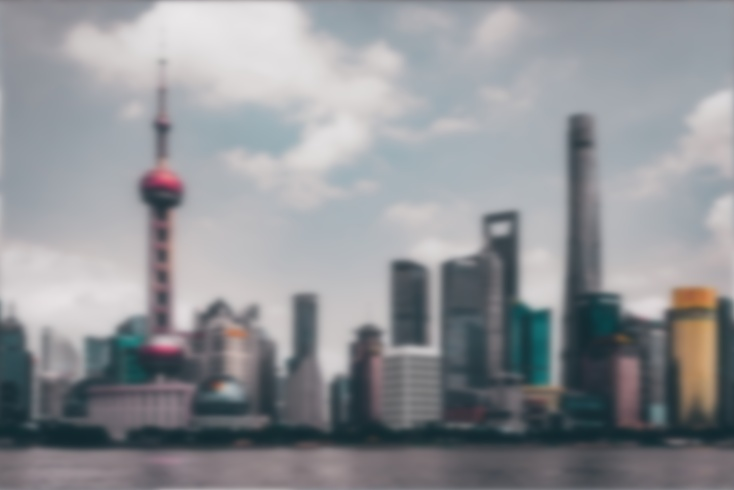
\includegraphics[width=0.9\textwidth]{output/1.1_turbulence.jpg}
            \end{minipage}
        }
                \subfigure[k = 0.01]{
            \begin{minipage}[t]{0.35\linewidth}
            \centering
            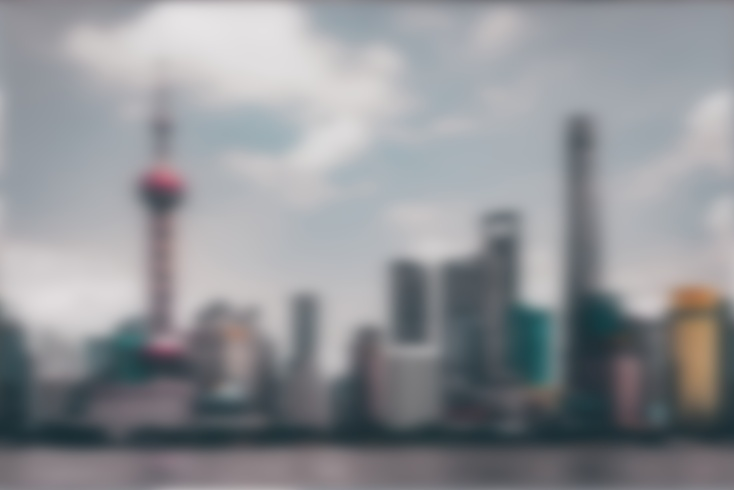
\includegraphics[width=0.9\textwidth]{output/1.1_turbulence_0.01.jpg}
            \end{minipage}
        }
        \centering
        \caption{大气湍流模型}\label{fig:digit}
  \end{figure}

\subsubsection*{运动模糊模型}

    \begin{figure}[htbp]
        \centering
        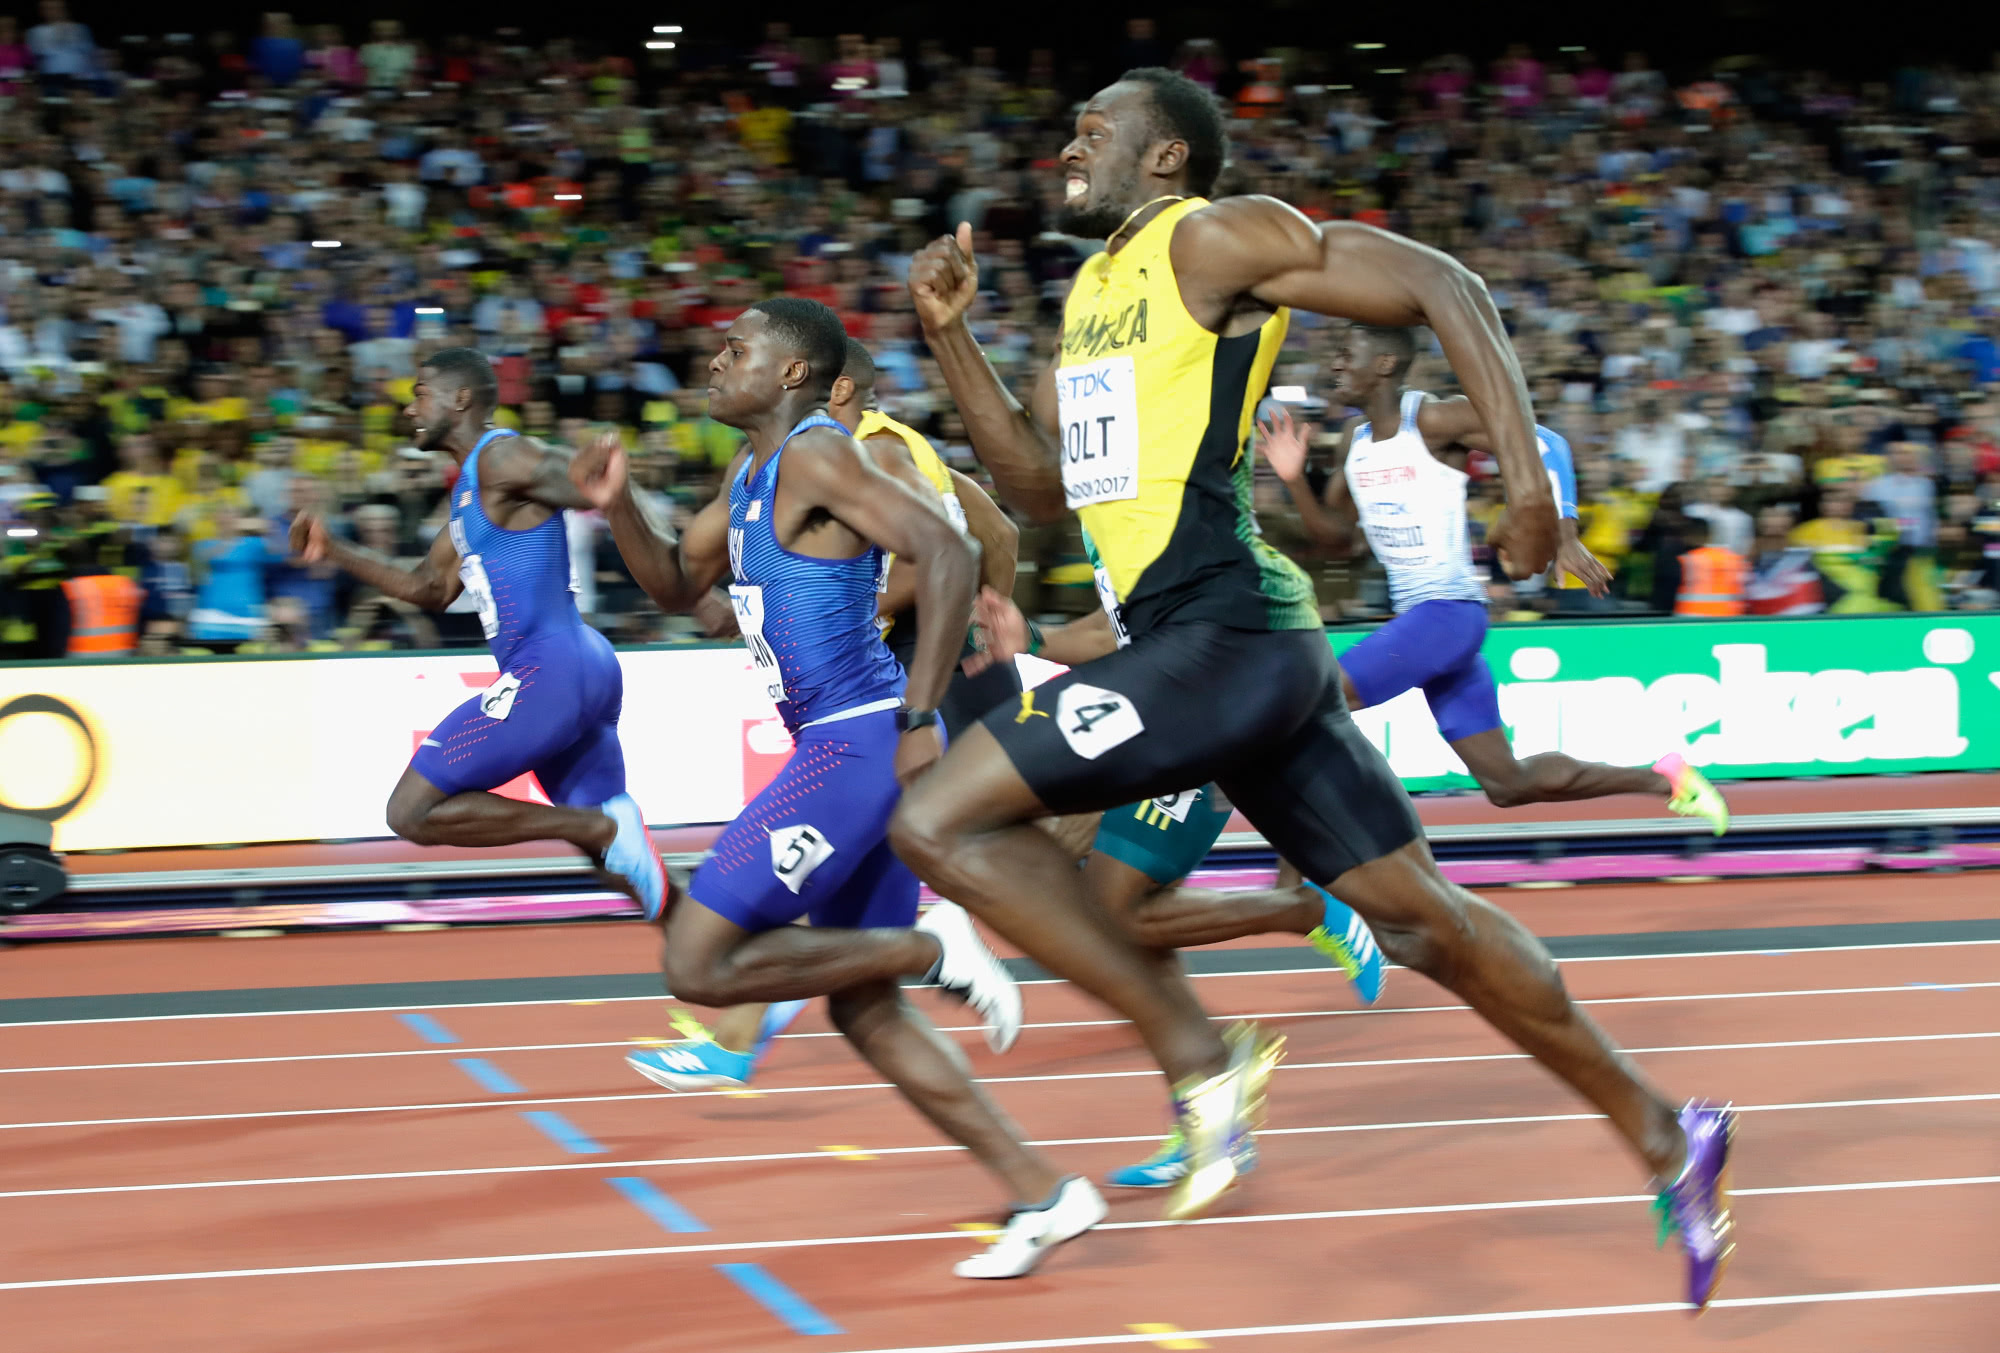
\includegraphics[width=0.4\textwidth]{input/2_1.jpeg}
        \caption{原图}
  \end{figure}

\newpage
    \begin{figure}[htbp]
        \centering
        \subfigure[移动方向为 $90$ 度]{
            \begin{minipage}[t]{0.4\linewidth}
            \centering
            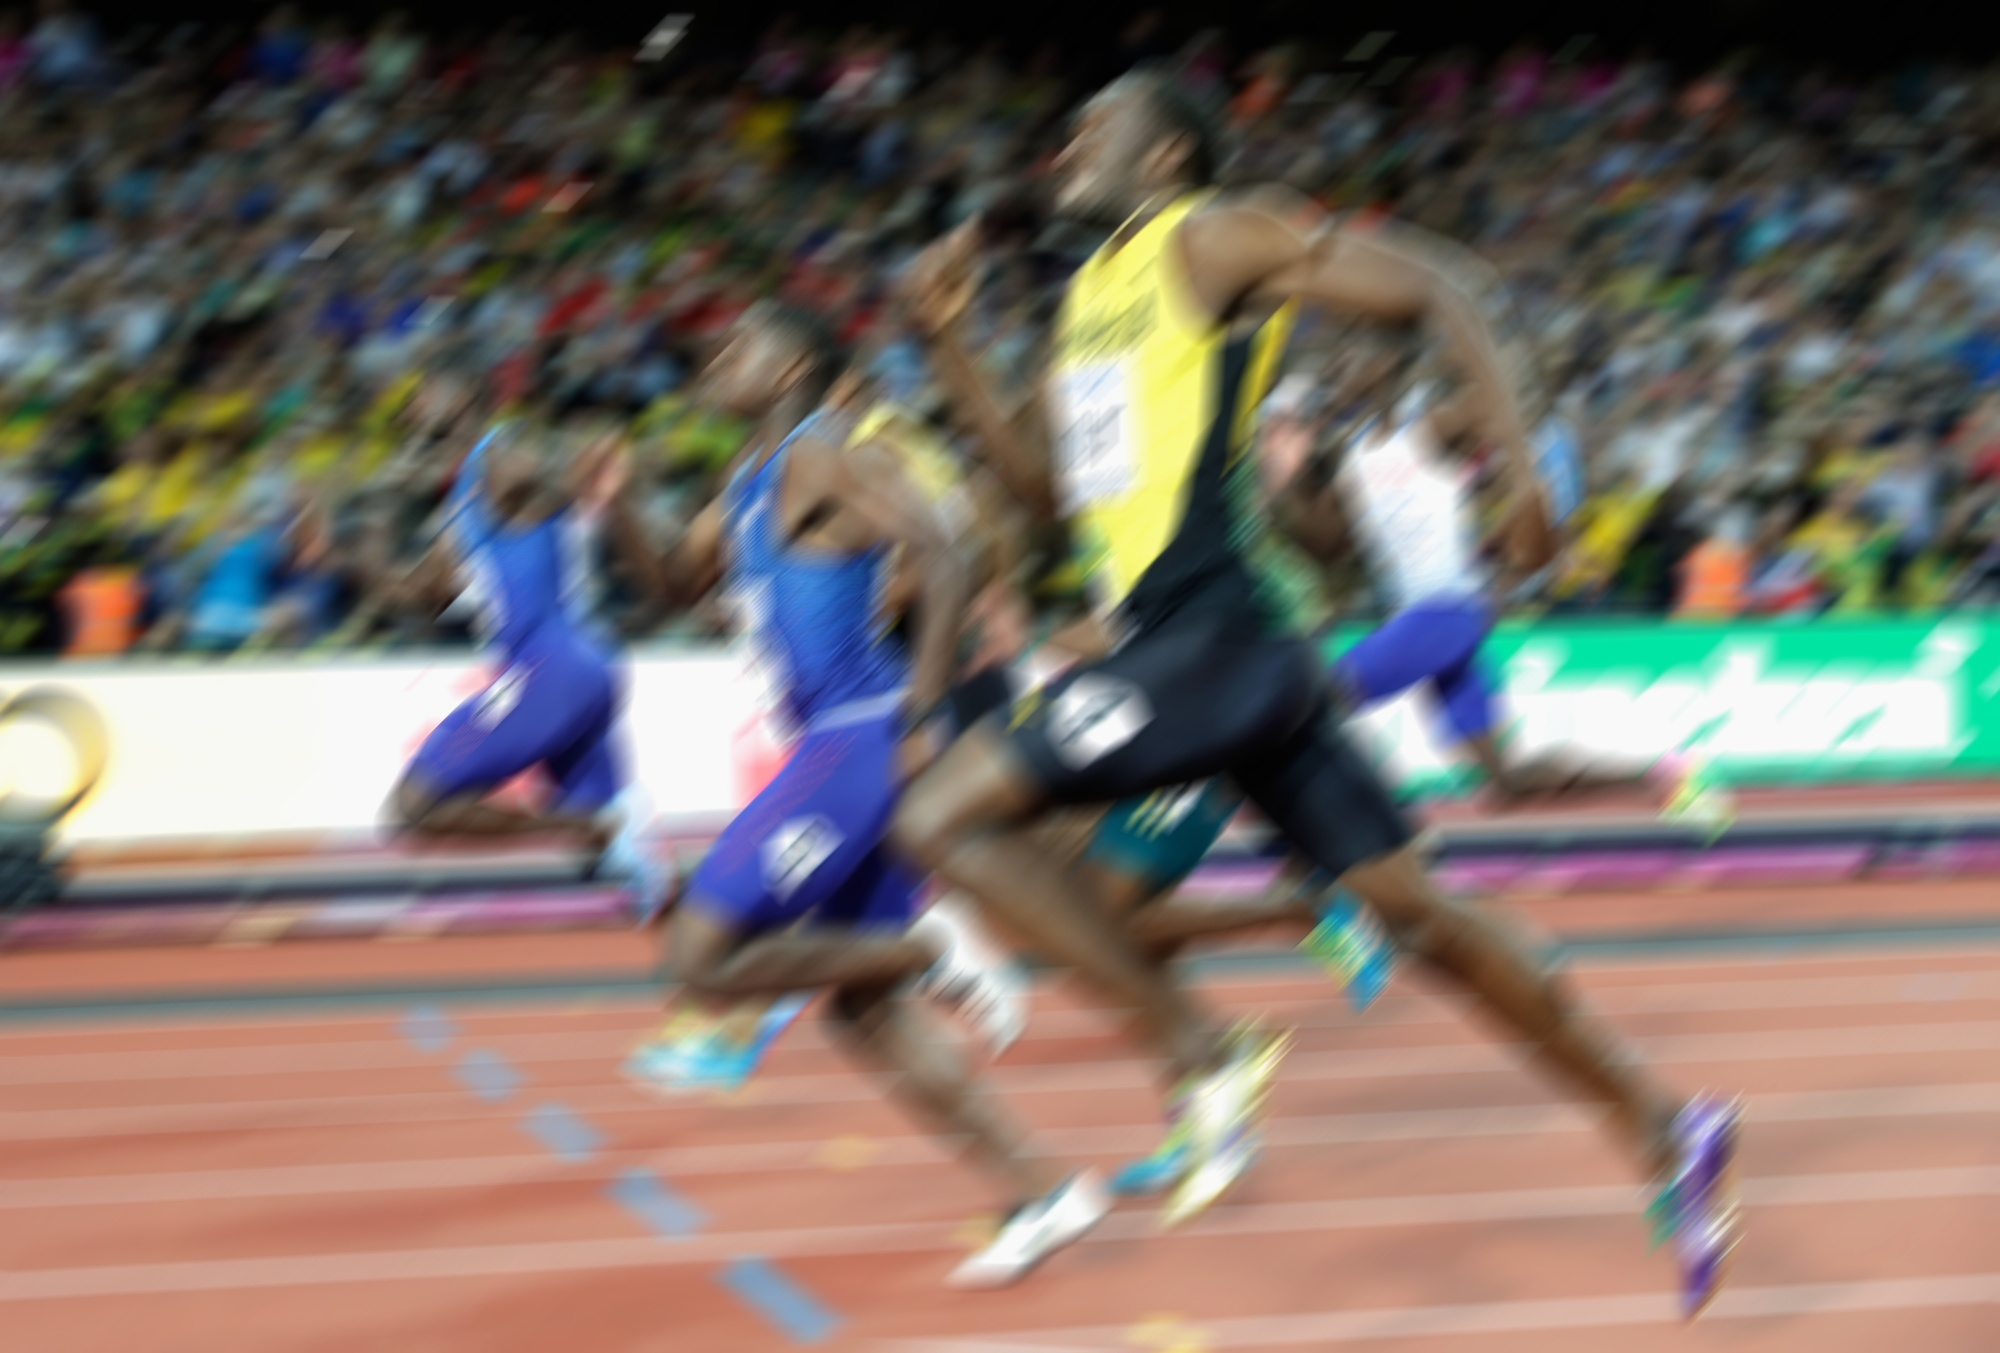
\includegraphics[width=0.9\textwidth]{output/output_2_1_30_90.jpg}
        \end{minipage}
        }
        \subfigure[傅里叶频谱]{
            \begin{minipage}[t]{0.4\linewidth}
            \centering
            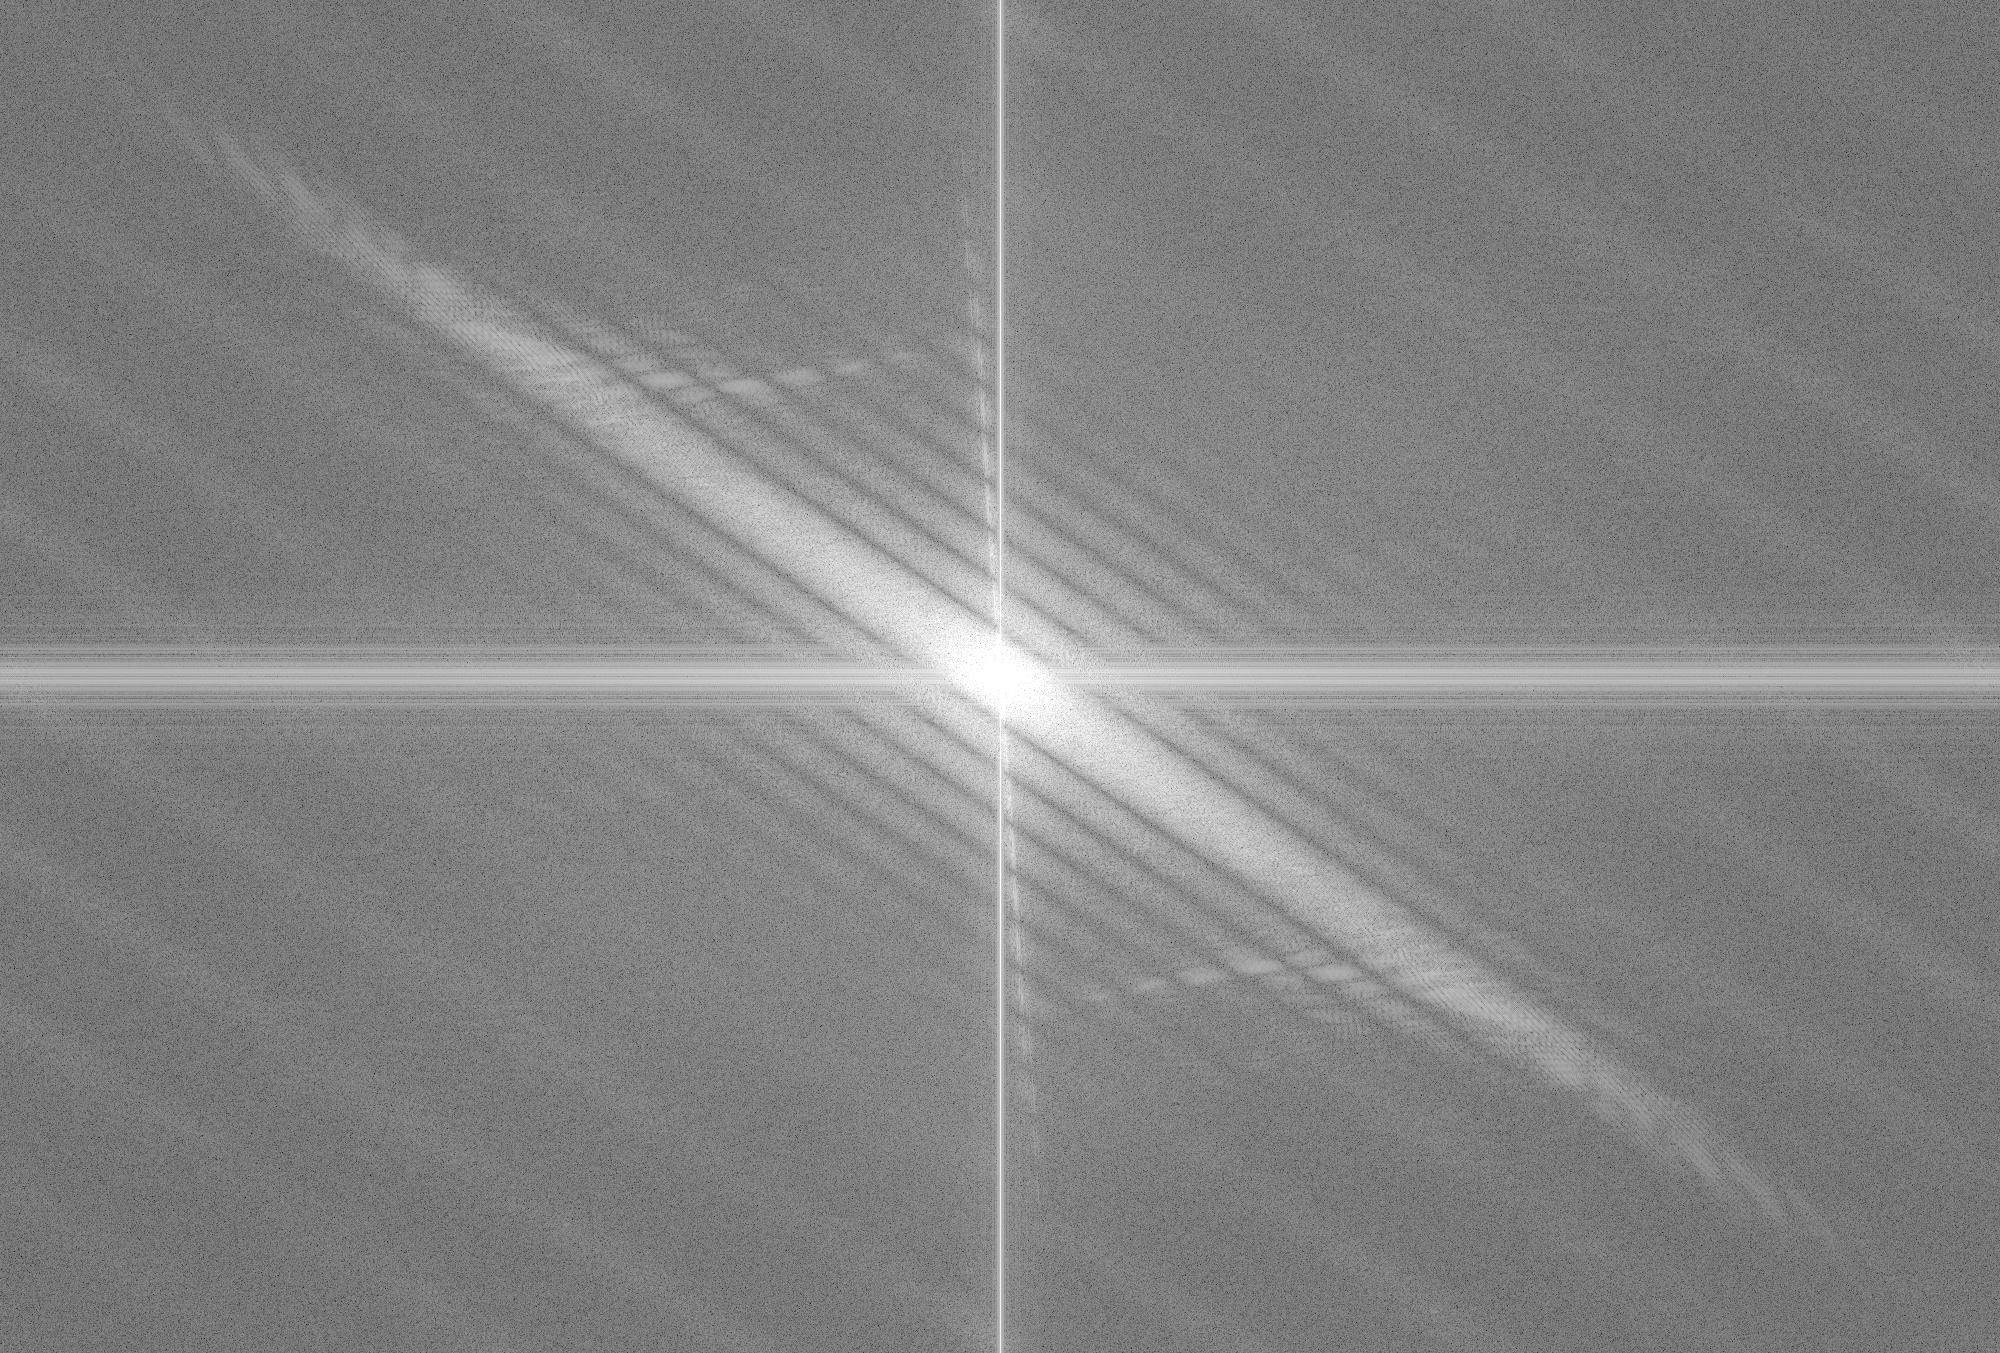
\includegraphics[width=0.9\textwidth]{output/output_2_1_30_90_fft.jpg}
            \end{minipage}
        }
        \centering
        \caption{运动模糊模型}\label{fig:digit}
  \end{figure}

    \begin{figure}[htbp]
        \centering
        \subfigure[移动方向为 $45$ 度]{
            \begin{minipage}[t]{0.4\linewidth}
            \centering
            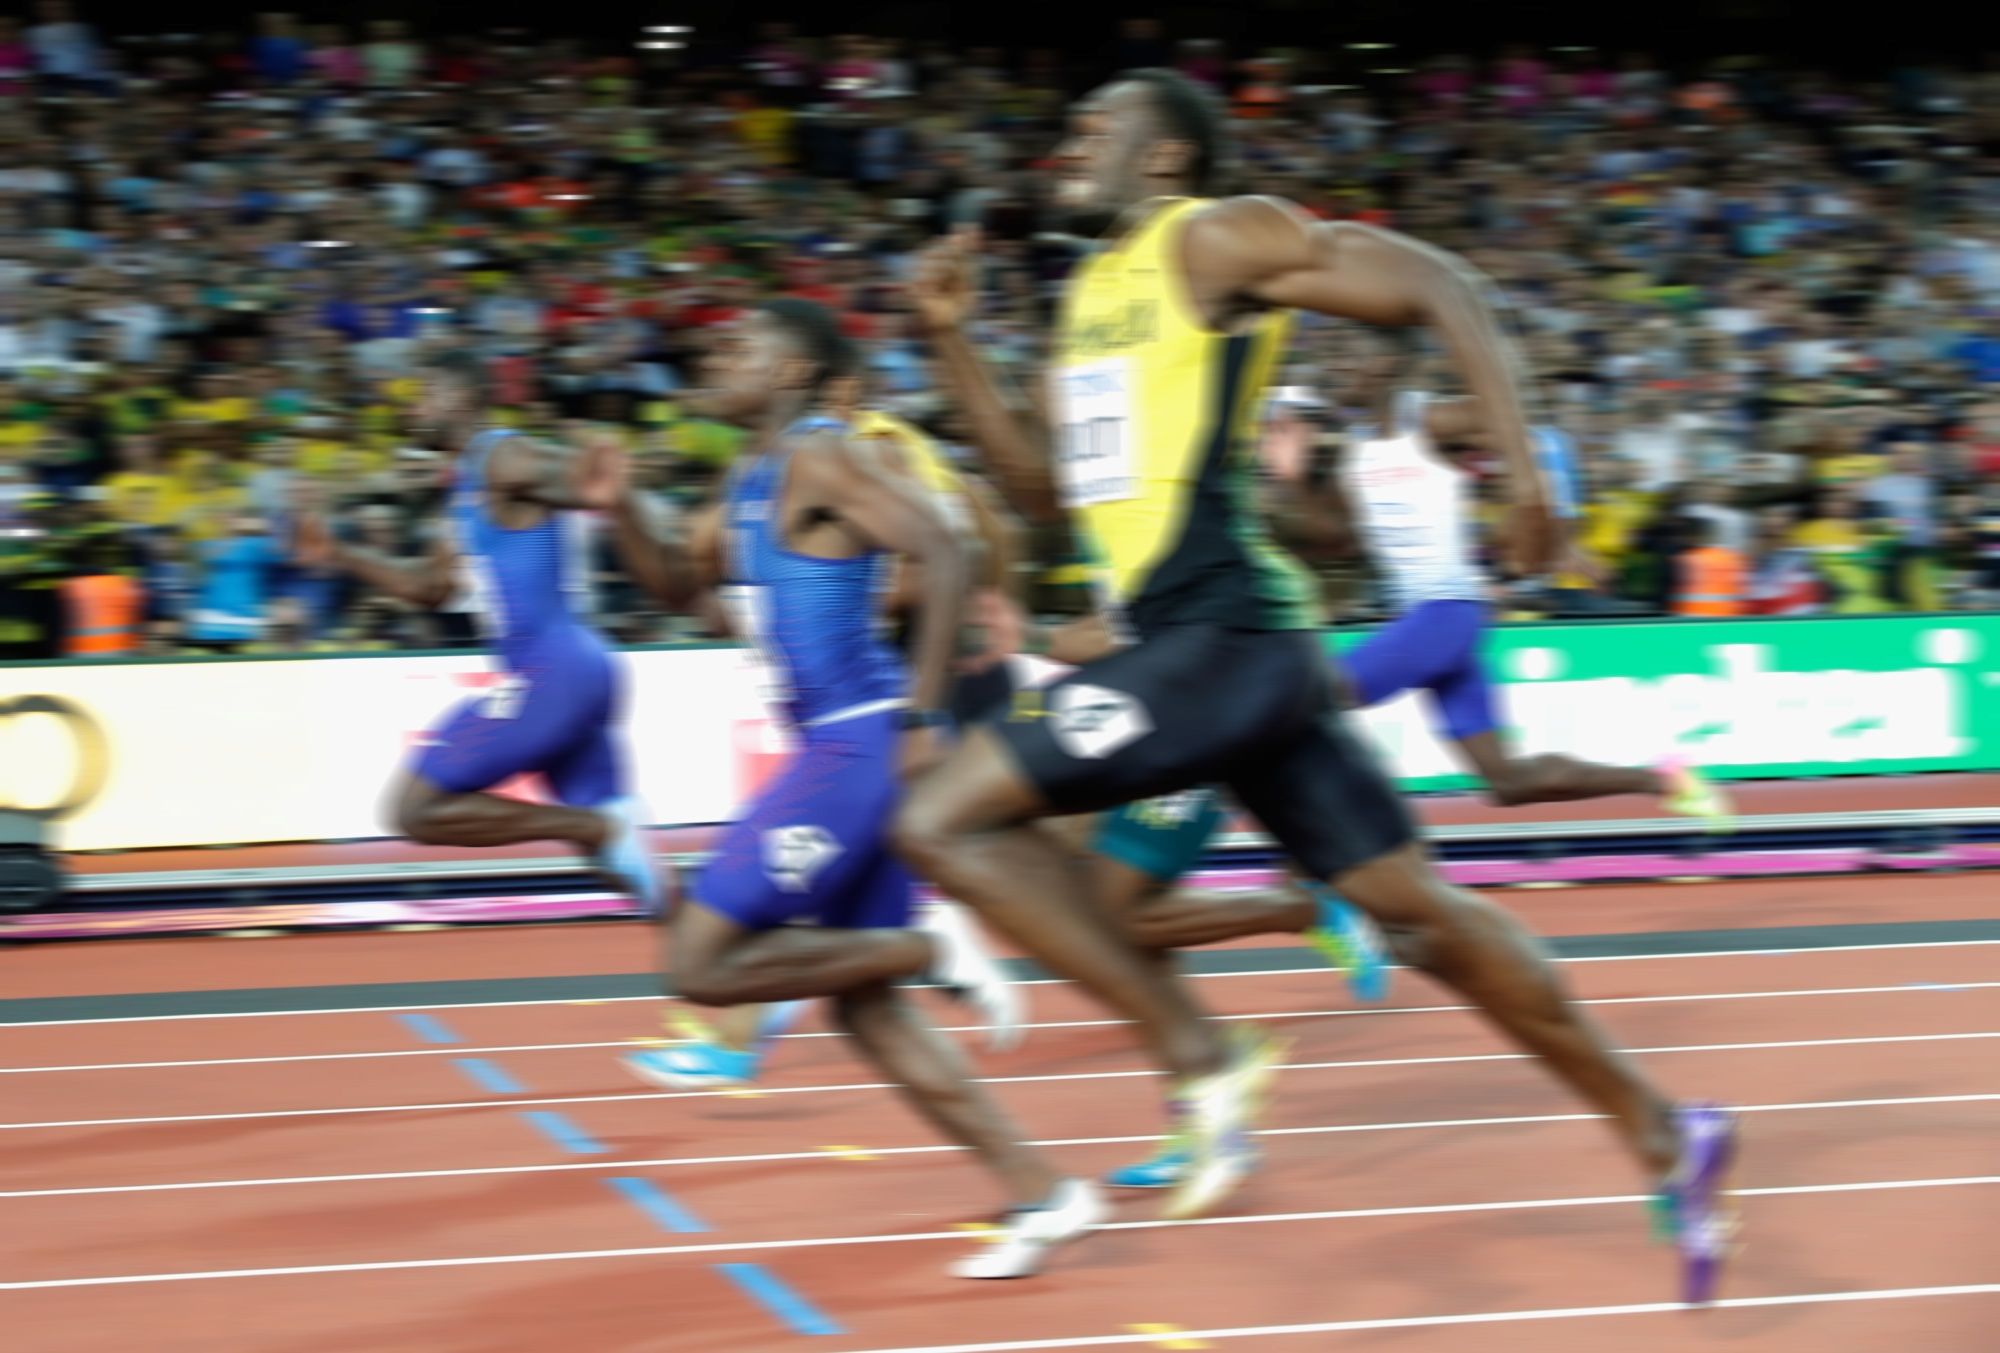
\includegraphics[width=0.9\textwidth]{output/output_2_1_30_45.jpg}
        \end{minipage}
        }
        \subfigure[傅里叶频谱]{
            \begin{minipage}[t]{0.4\linewidth}
            \centering
            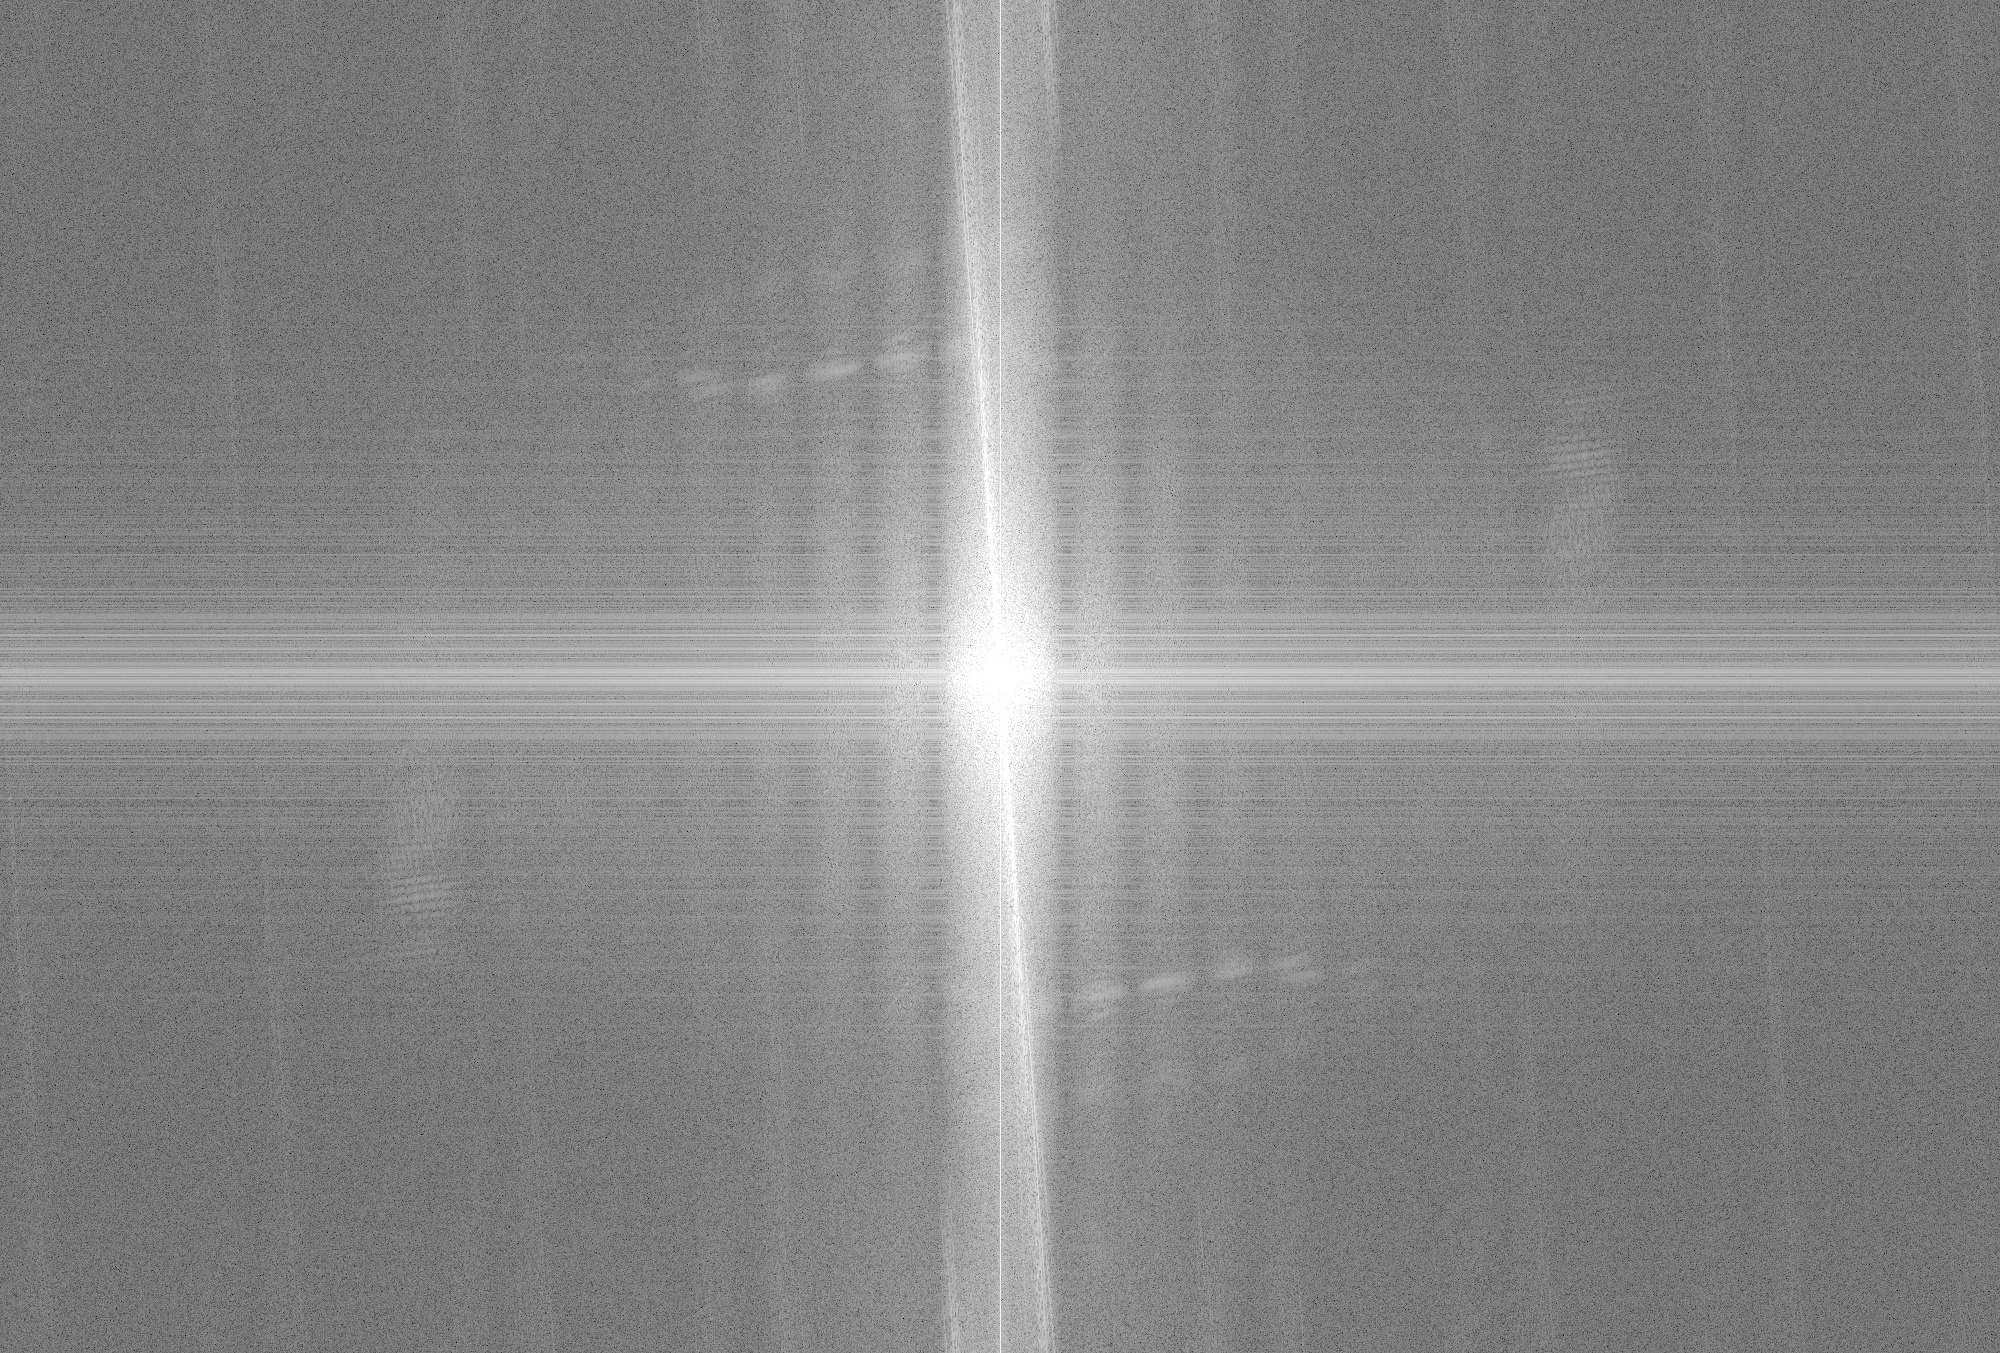
\includegraphics[width=0.9\textwidth]{output/output_2_1_30_45_fft.jpg}
            \end{minipage}
        }
        \centering
        \caption{运动模糊模型}\label{fig:digit}
  \end{figure}
  
\newpage

\subsection*{图像恢复}

\subsubsection*{直接逆滤波}

    \begin{figure}[htbp]
        \centering
        \subfigure[退化图]{
            \begin{minipage}[t]{0.35\linewidth}
            \centering
            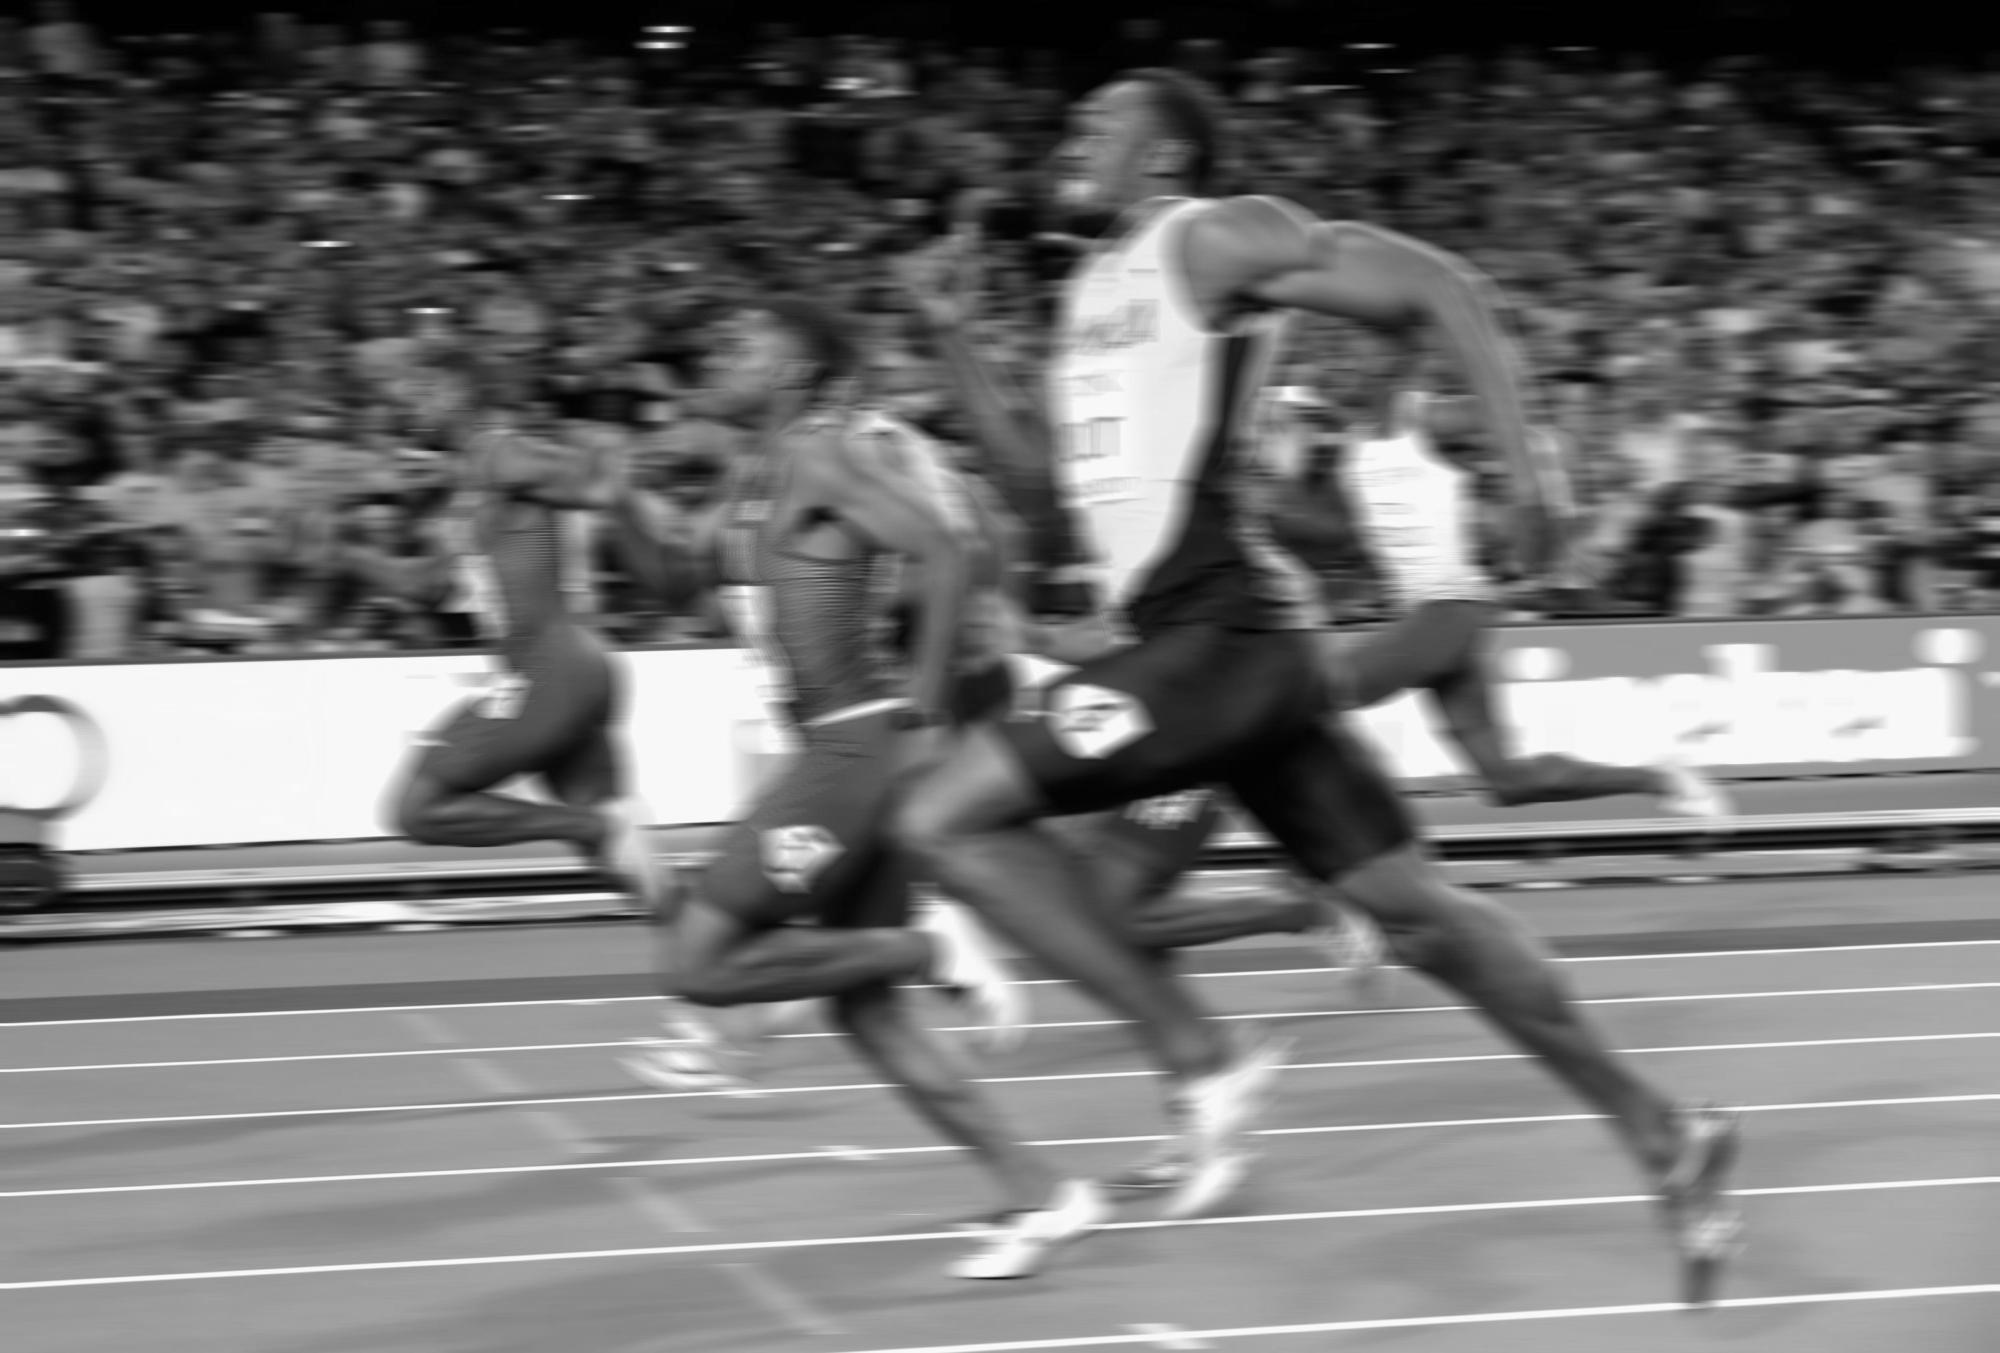
\includegraphics[width=0.9\textwidth]{output/2_motion_process.jpg}
        \end{minipage}
        }
        \subfigure[恢复图]{
            \begin{minipage}[t]{0.35\linewidth}
            \centering
            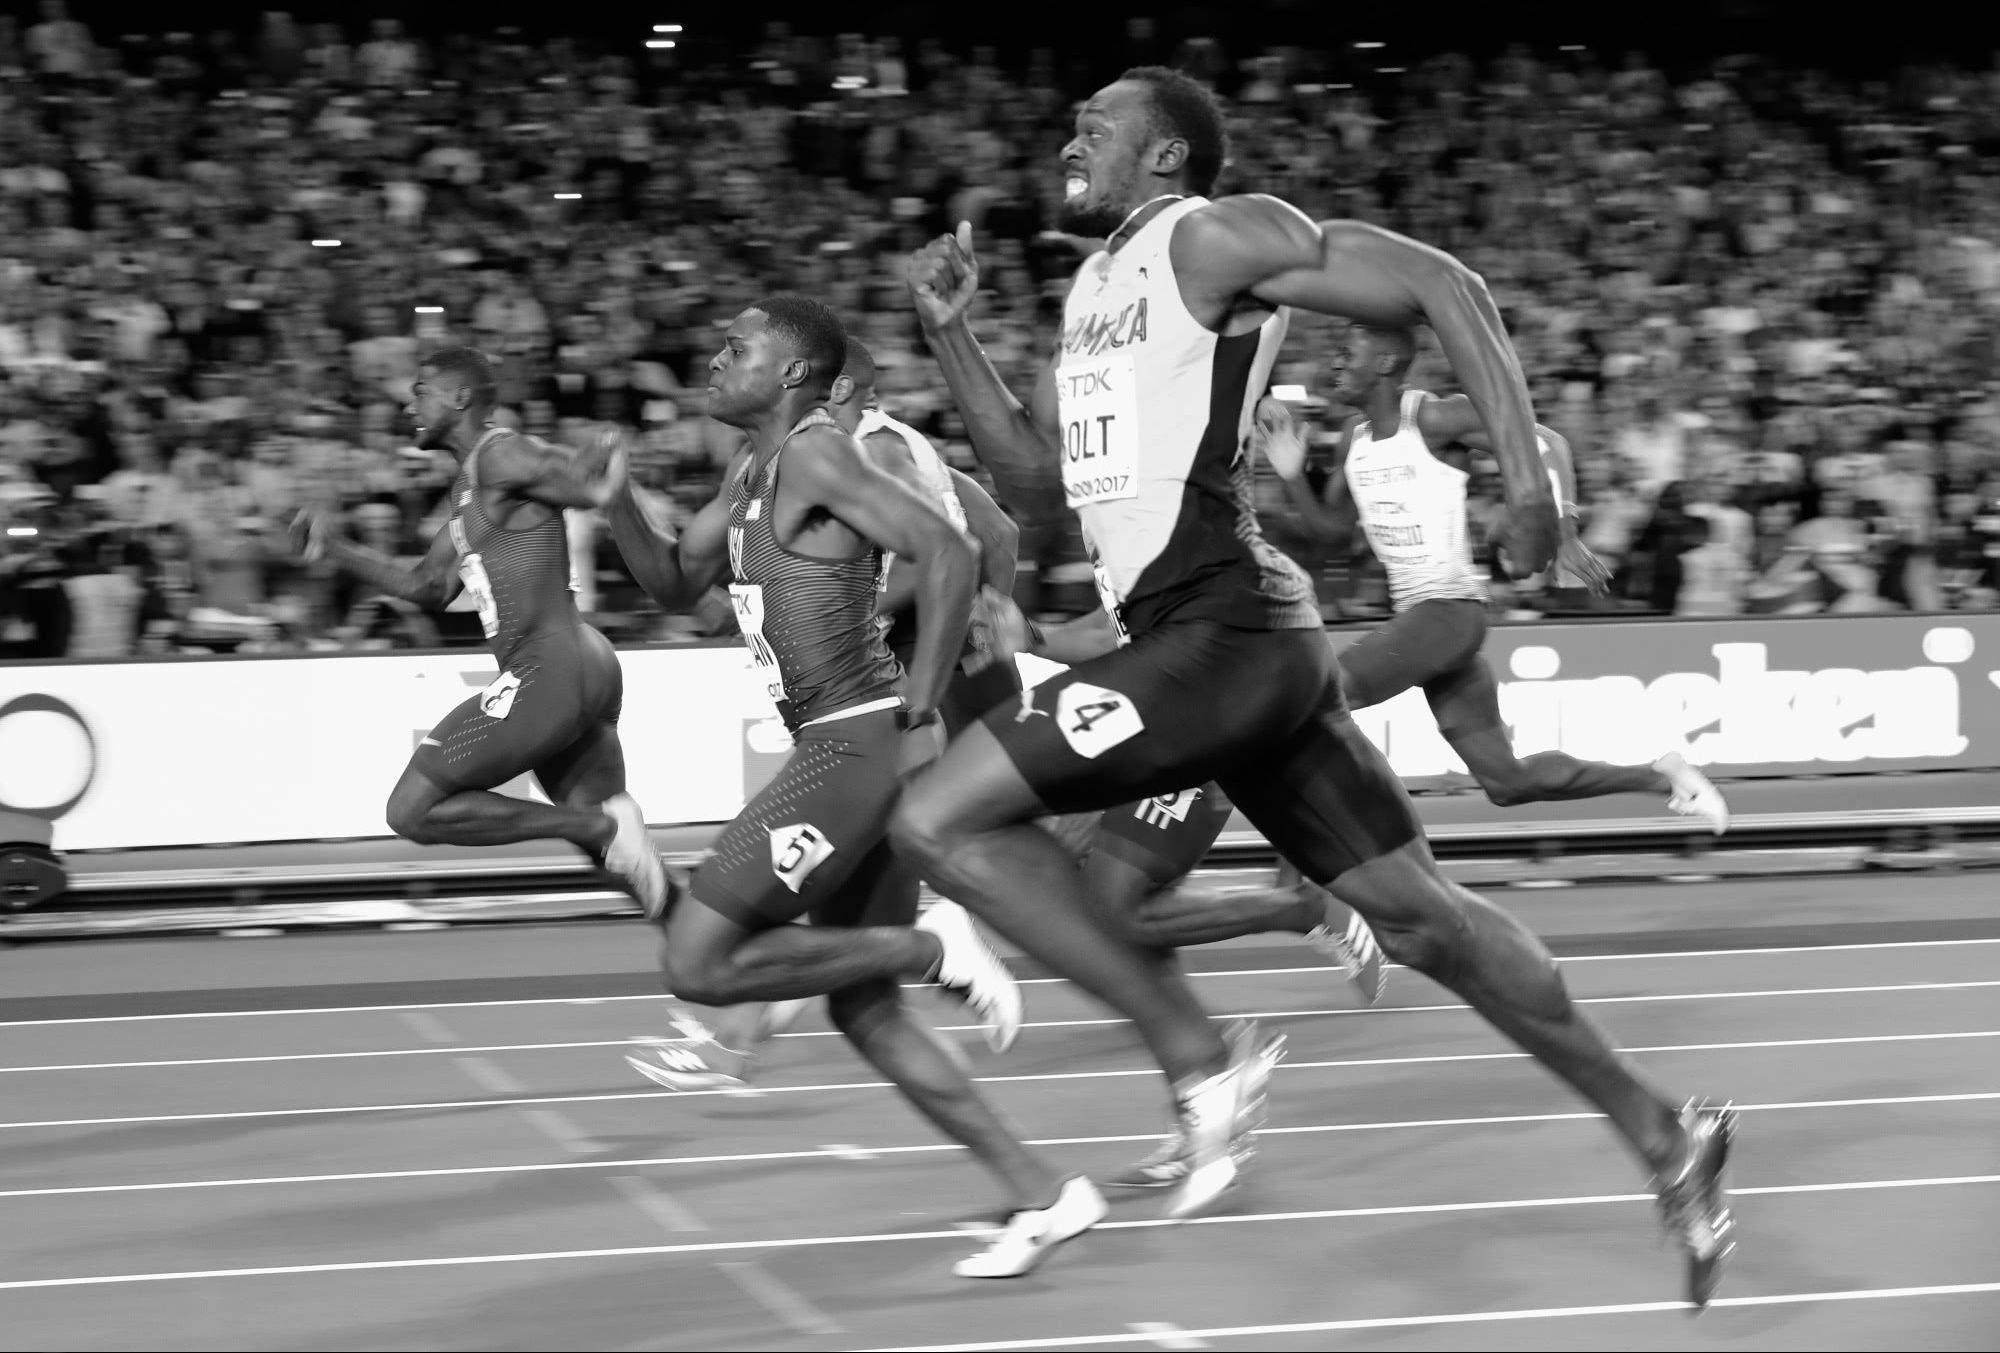
\includegraphics[width=0.9\textwidth]{output/2_inverse.jpg}
            \end{minipage}
        }
        \centering
        \caption{运动模糊模型}\label{fig:digit}
  \end{figure}
  


\subsubsection*{维纳滤波}

    \begin{figure}[htbp]
        \centering
        \subfigure[退化图]{
            \begin{minipage}[t]{0.36\linewidth}
            \centering
            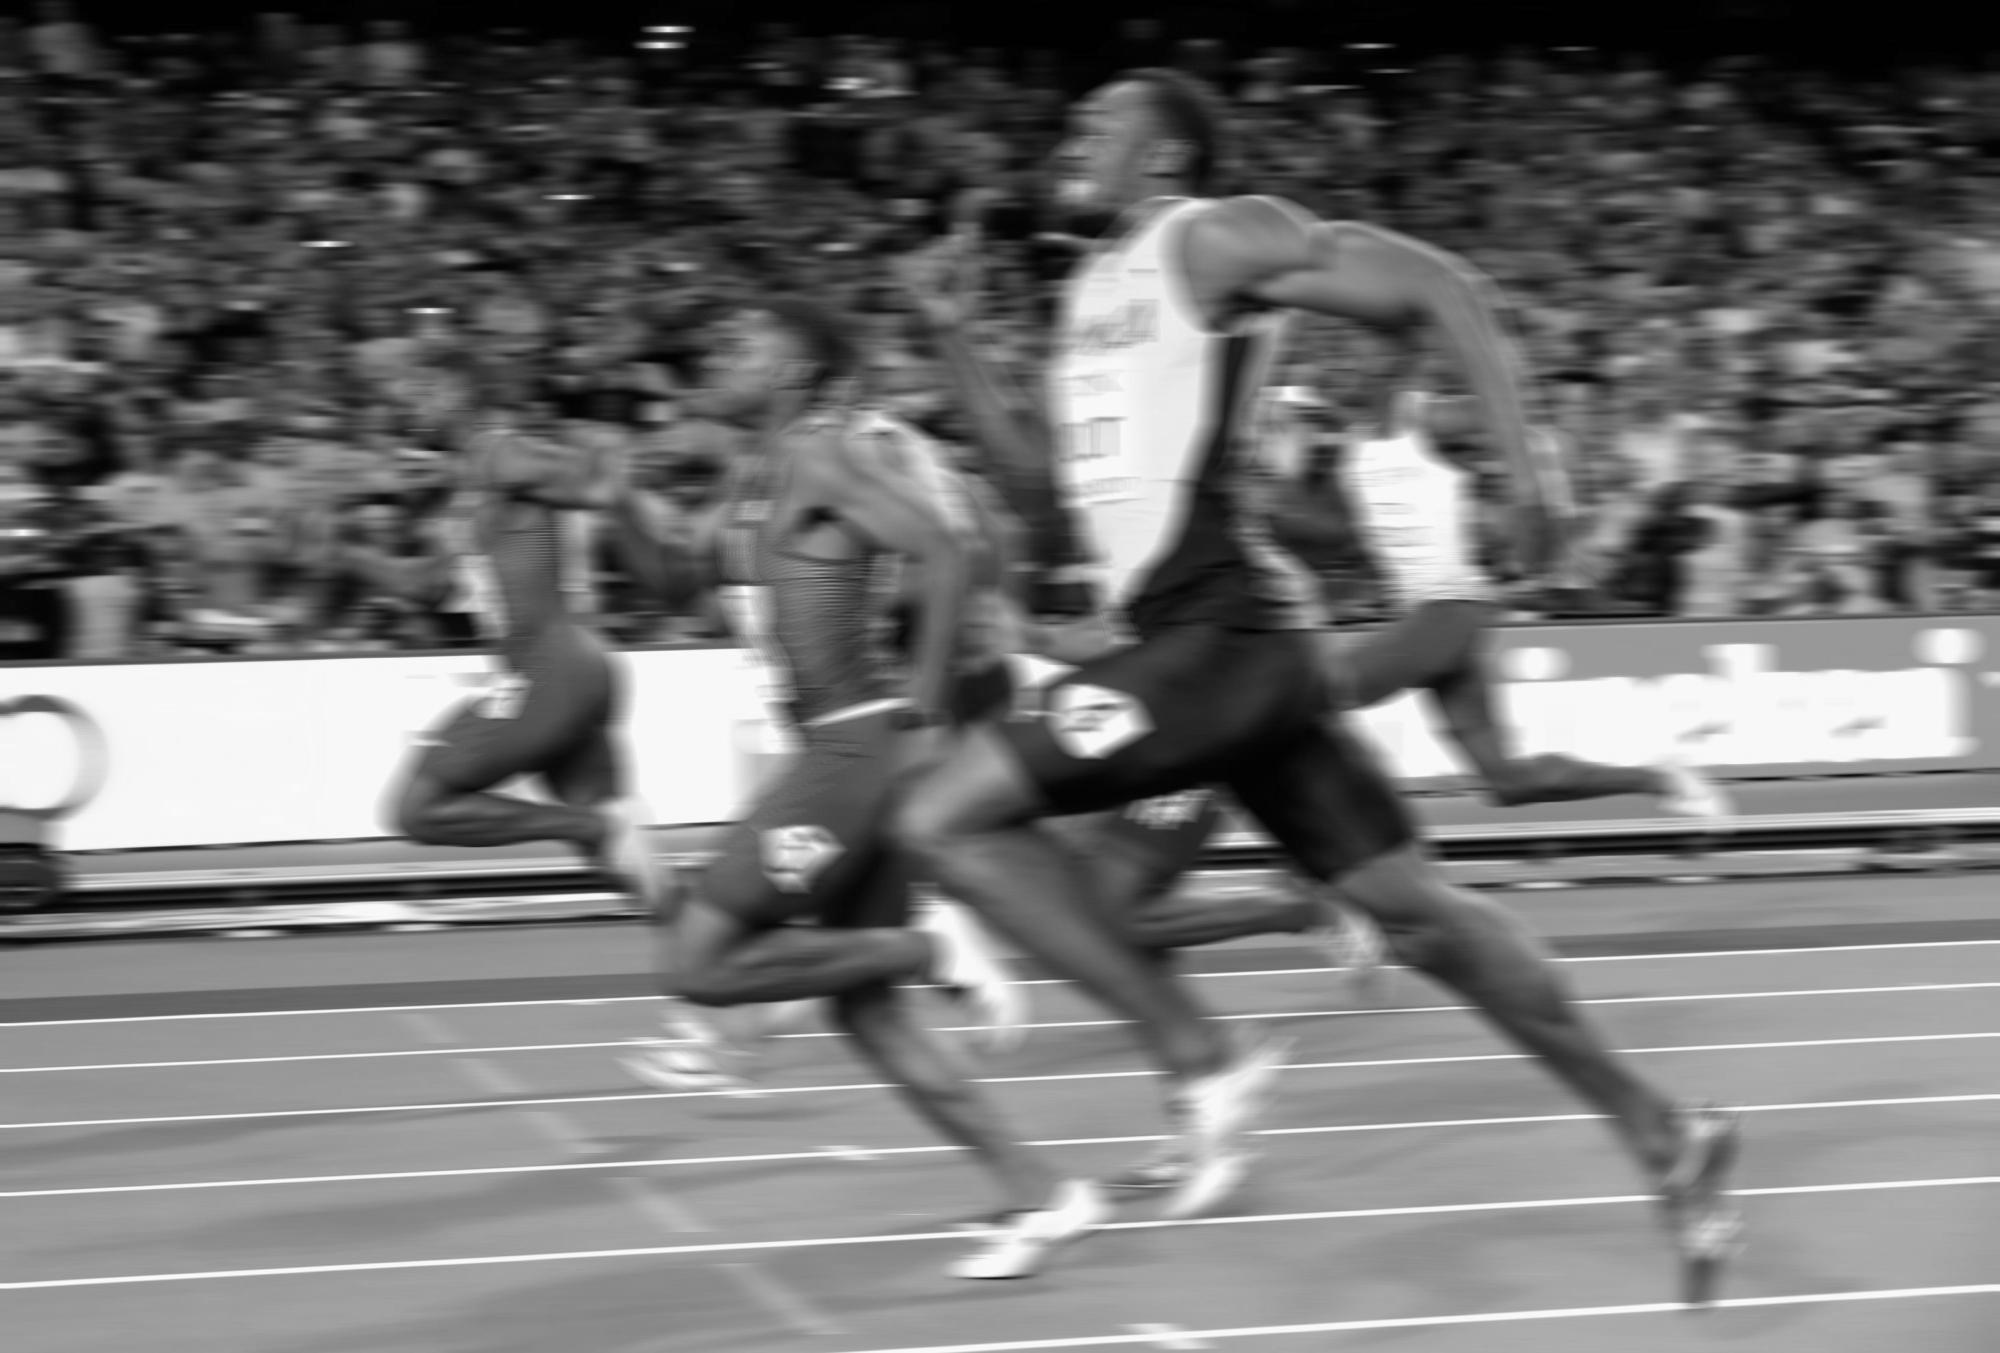
\includegraphics[width=0.9\textwidth]{output/2_motion_process.jpg}
        \end{minipage}
        }
        \subfigure[恢复图,参数 = $1$]{
            \begin{minipage}[t]{0.36\linewidth}
            \centering
            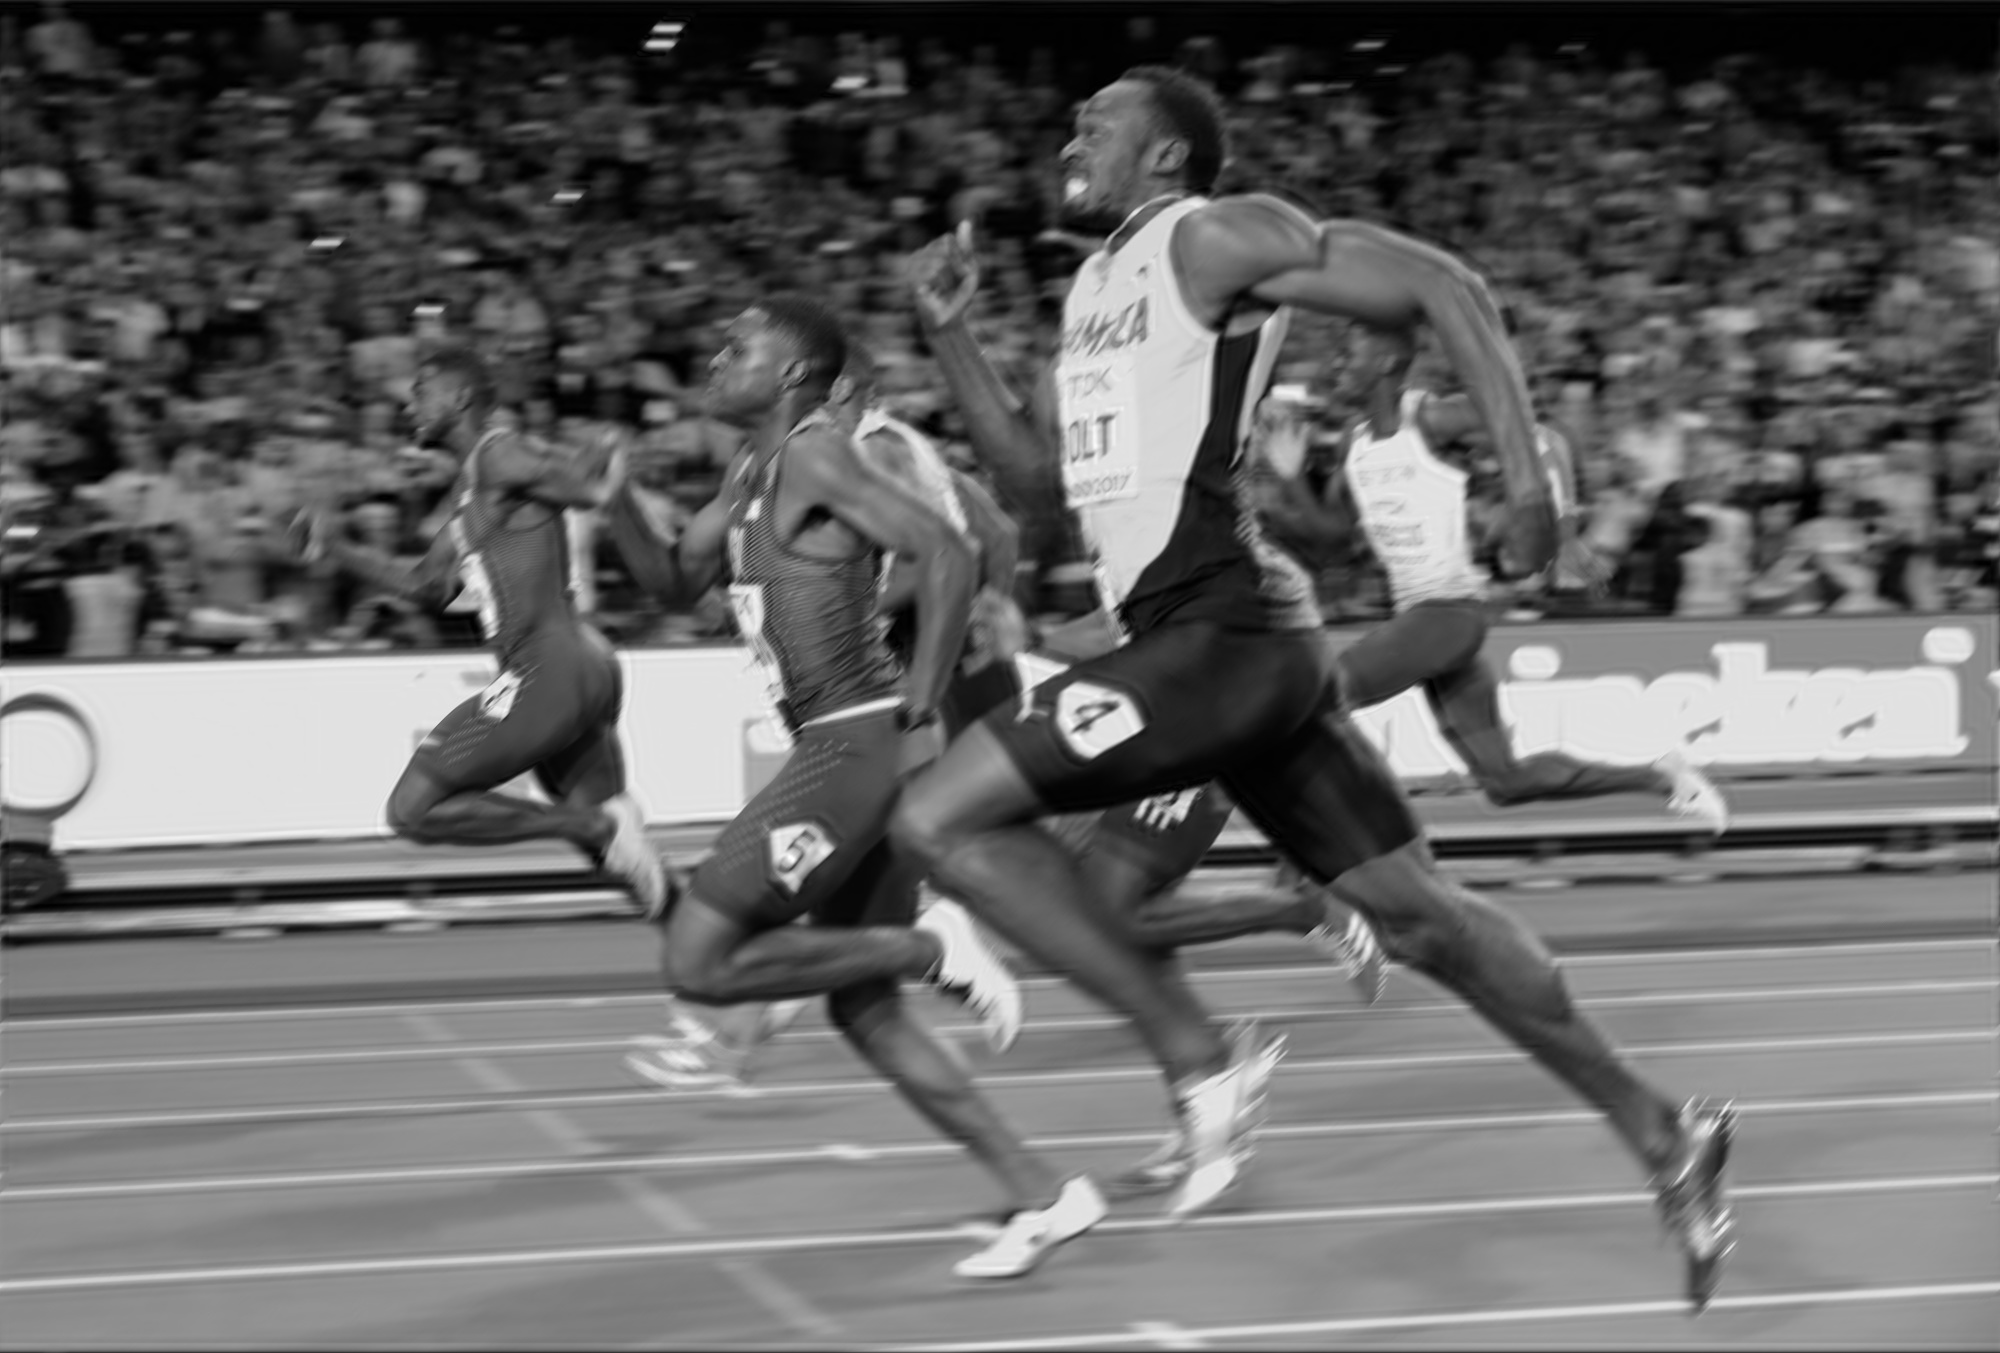
\includegraphics[width=0.9\textwidth]{output/2_wiener_1.jpg}
            \end{minipage}
        }
        \subfigure[恢复图,参数 = $0.1$]{
            \begin{minipage}[t]{0.36\linewidth}
            \centering
            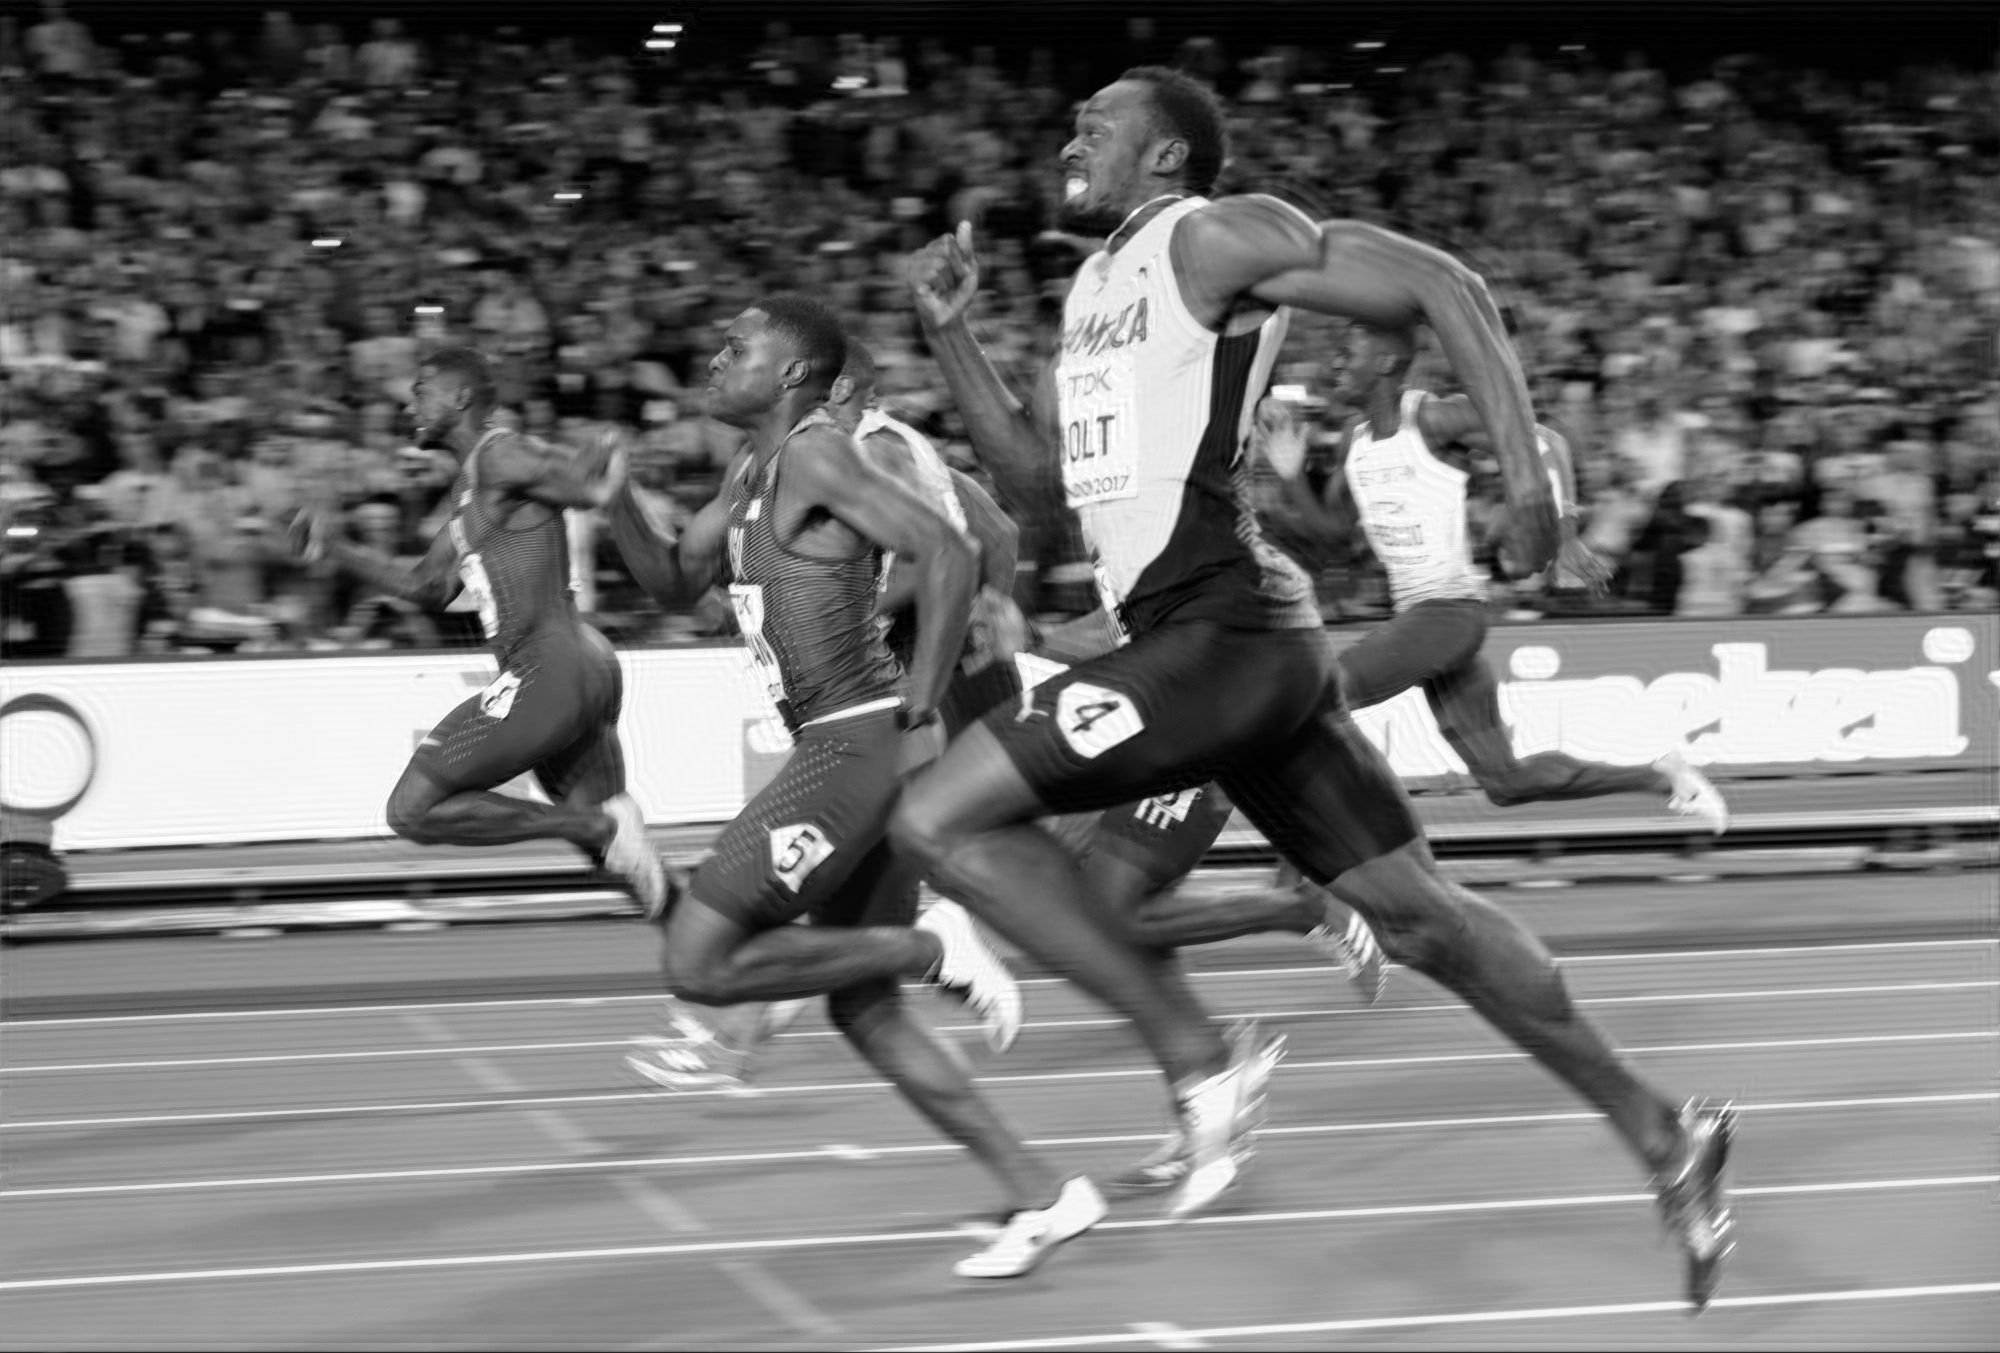
\includegraphics[width=0.9\textwidth]{output/2_wiener_01.jpg}
            \end{minipage}
        }
        \subfigure[恢复图,参数 = $0.01$]{
            \begin{minipage}[t]{0.36\linewidth}
            \centering
            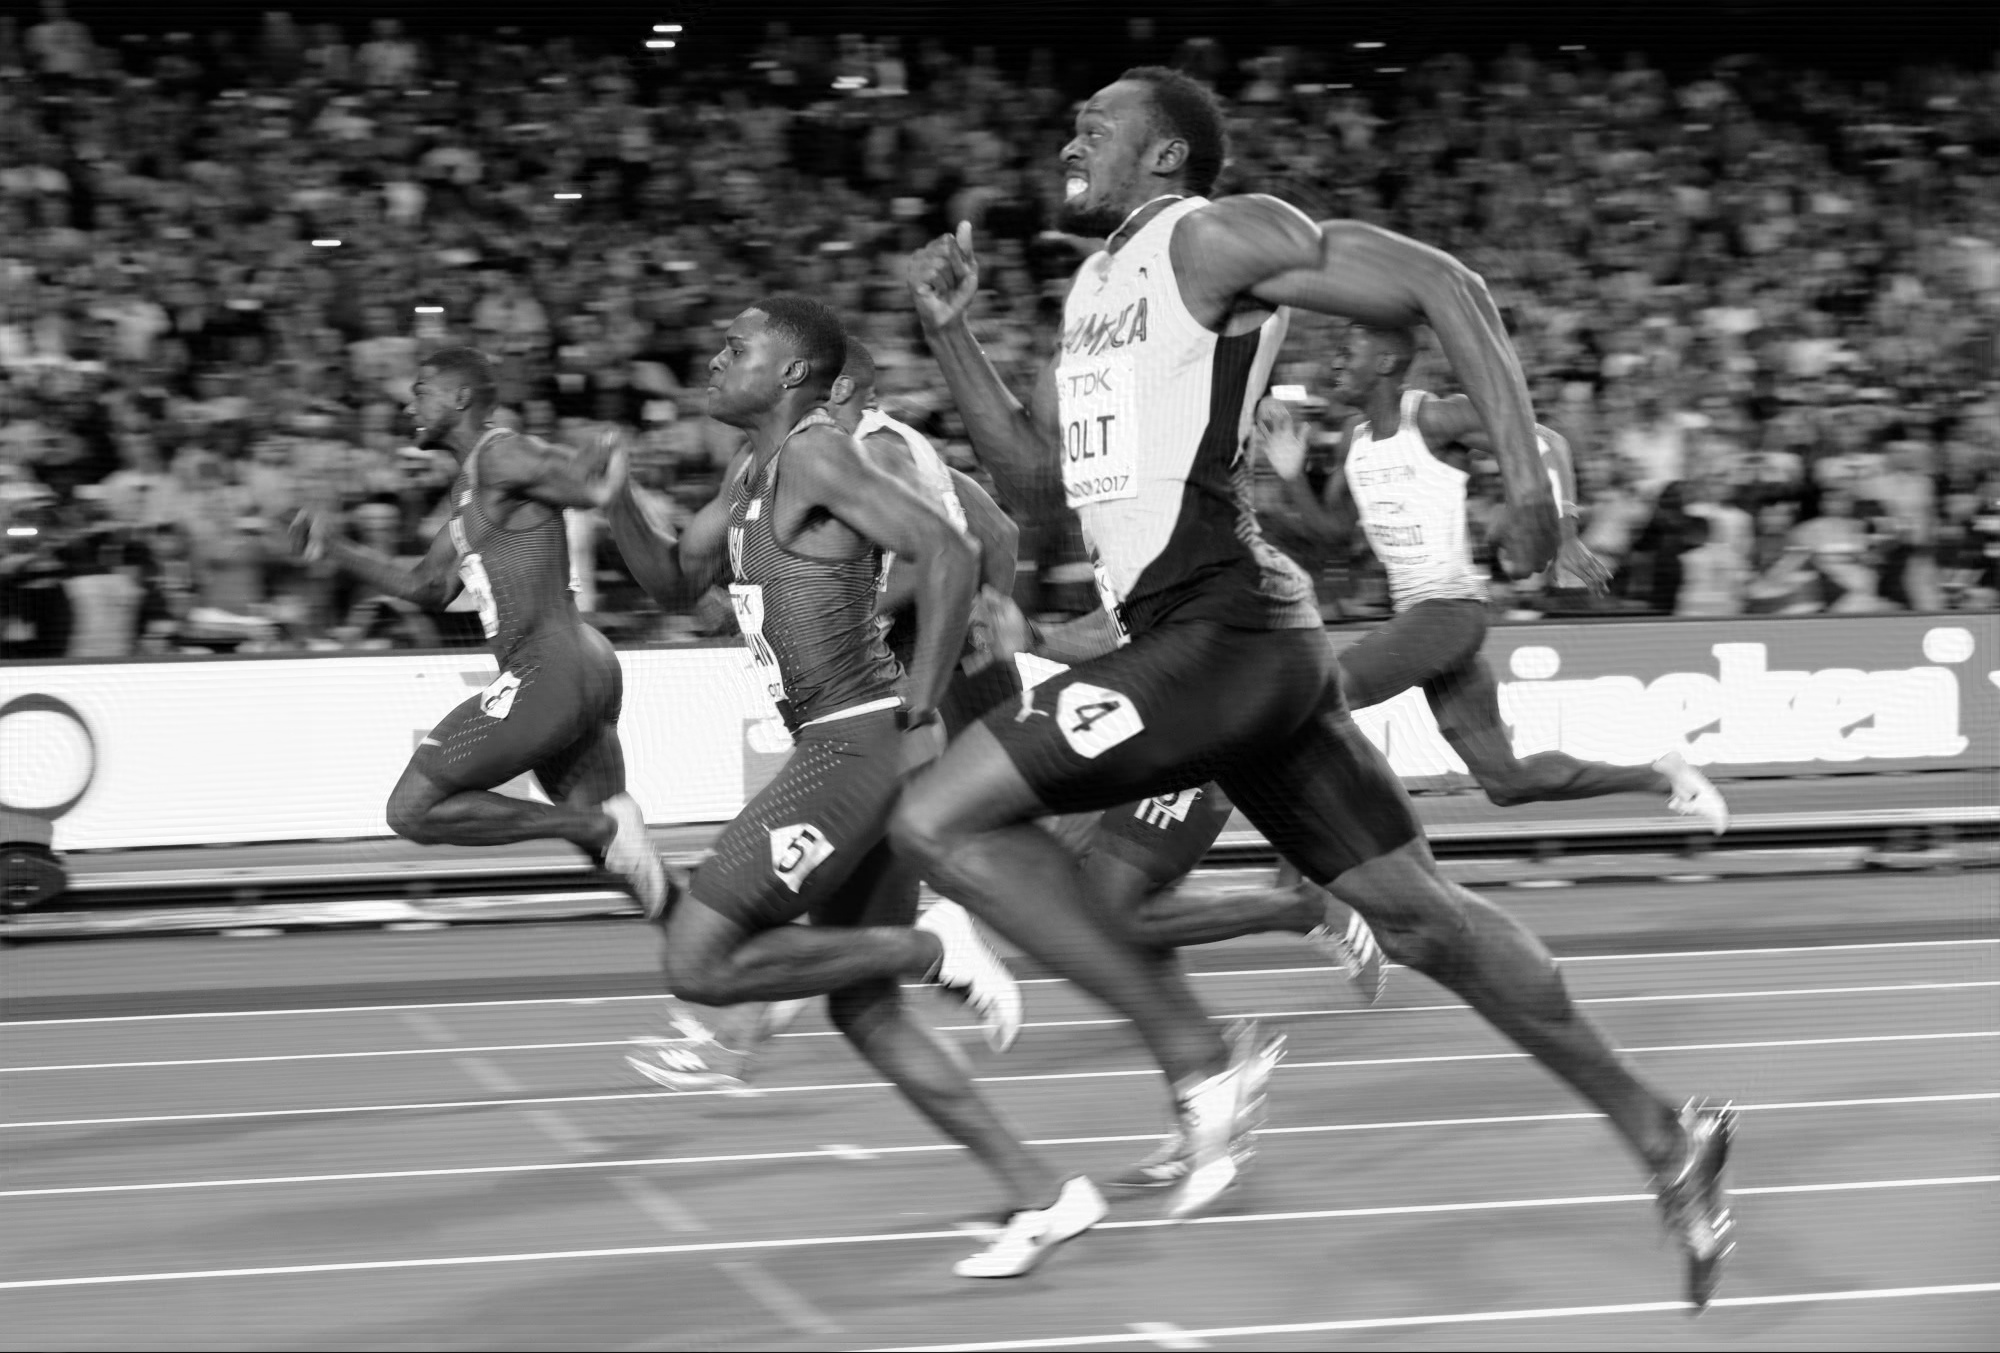
\includegraphics[width=0.9\textwidth]{output/2_wiener_001.jpg}
            \end{minipage}
        }
        \centering
        \caption{运动模糊模型}\label{fig:digit}
  \end{figure}

\newpage

\subsubsection*{约束最小二乘方滤波器}

    \begin{figure}[htbp]
        \centering
        \subfigure[退化图]{
            \begin{minipage}[t]{0.4\linewidth}
            \centering
            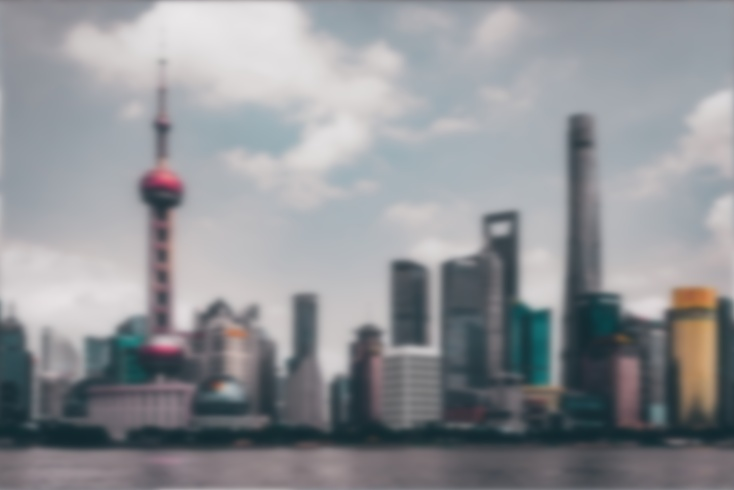
\includegraphics[width=0.9\textwidth]{output/1.1_turbulence.jpg}
        \end{minipage}
        }
        \subfigure[退化图经过约束最小二乘方滤波器]{
            \begin{minipage}[t]{0.4\linewidth}
            \centering
            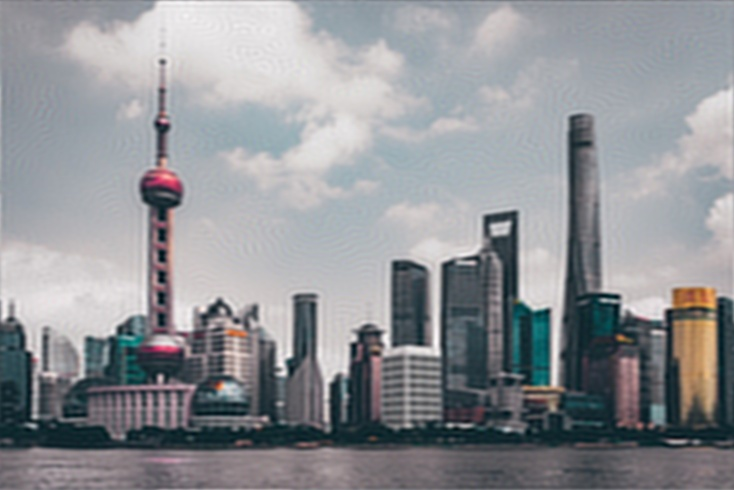
\includegraphics[width=0.9\textwidth]{output/1.1_recovered_CLS_nonoise.jpg}
            \end{minipage}
        }
        \subfigure[退化+噪声图]{
            \begin{minipage}[t]{0.4\linewidth}
            \centering
            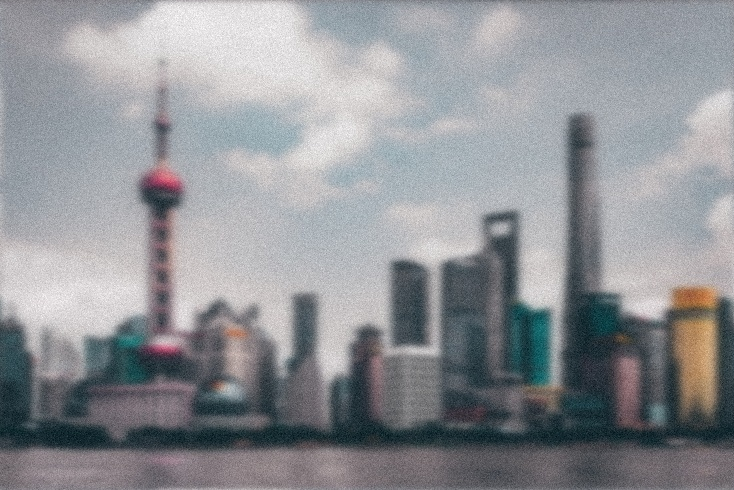
\includegraphics[width=0.9\textwidth]{output/1.1_turbulence_noise.jpg}
        \end{minipage}
        }
        \subfigure[退化+噪声图经过约束最小二乘方滤波器]{
            \begin{minipage}[t]{0.4\linewidth}
            \centering
            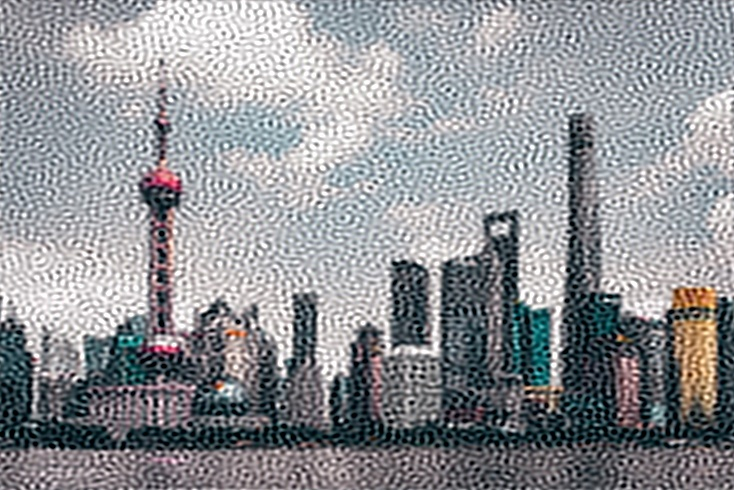
\includegraphics[width=0.9\textwidth]{output/1.1_recovered_CLS.jpg}
            \end{minipage}
        }
        \centering
        \caption{大气湍流模型恢复}\label{fig:digit}
  \end{figure}


\section{主要核心代码}

在代码部分,我们为了将退化和恢复写在了一起,即对图片进行相应的退后后,在利用不同的恢复方法对图片进行恢复。所以代码部分主要分成两部分内容。

\paragraph{大气湍流模型及其恢复}

\lstset{language=python}
\begin{lstlisting}
import matplotlib.pyplot as plt
import numpy as np
from numpy import fft
import cv2
import time


# 退化函数,用于逆滤波
Huv = 0

def psf2otf(psf, shape):
	"""
	将 PSF 转化为 OTF
	:param psf: 原 PSF
	:param shape: 图像对应的大小
	:return: OTF
	"""
	inshape = psf.shape
	idx, idy = np.indices(np.asarray(inshape))
	# psf = zero_pad(psf, shape, position='corner')
	pad = np.zeros(shape)
	pad[idx, idy] = psf
	psf = pad
	# Circularly shift OTF so that the 'center' of the PSF is
	# [0,0] element of the array
	for axis, axis_size in enumerate(inshape):
		psf = np.roll(psf, -int(axis_size / 2), axis=axis)
	# Compute the OTF
	otf = np.fft.fft2(psf)
	# Estimate the rough number of operations involved in the FFT
	# and discard the PSF imaginary part if within roundoff error
	# roundoff error  = machine epsilon = sys.float_info.epsilon
	# or np.finfo().eps
	n_ops = np.sum(psf.size * np.log2(psf.shape))
	otf = np.real_if_close(otf, tol=n_ops)
	return fft.fftshift(otf)

def turbulence(image, k=0.0025):
	"""
	大气退化模型估计
	:param image: 原图像
	:param k: 退化函数中的 k 值
	:return: 退化图像
	"""
	global Huv
	img_h = image.shape[0]
	img_w = image.shape[1]
	center = [int(img_h/2), int(img_w/2)]
	H = np.zeros((img_h, img_w))
	print("Calculating degrade function...")
	# 计算退化函数
	for u in range(img_h):
		for v in range(img_w):
			temp = (u - center[0]) ** 2 + (v - center[1]) ** 2
			# H[u][v] = np.exp((-k) * (temp ** (float(5) / 6)))
			H[u][v] = np.e ** ((-k) * (temp ** (float(5) / 6)))
	# 对三个颜色通道进行处理
	Huv = H
	R, G, B = cv2.split(image)
	channels = [R, G, B]
	out = []
	for one in channels:
		print("Fourier transform...")
		ft = fft.fft2(one)
		ft = fft.fftshift(ft)
		thisout = ft * H
		thisout = fft.ifft2(fft.ifftshift(thisout))
		out.append(np.uint8(np.real(thisout)))
	return cv2.merge(out)

def add_noise_gussian(src, mean=0, var=0.001):
	"""
	添加高斯噪声
	:param src: 原图像
	:param mean: 均值
	:param var: 方差
	:return: 添加了噪声之后的图像
	"""
	# 生成随机高斯噪声
	noise = np.random.normal(mean, var ** 0.5, src.shape[:2])
	R, G, B = cv2.split(src)
	channels = [R, G, B]
	out = []
	for one in channels:
		one = one / 255 + noise
		np.clip(one, 0, 1)
		out.append(one * 255)
	return cv2.merge(out)


def recover_CLSF(image, H, gamma = 0.01):
	"""
	约束最小二乘方滤波 Constrained Least Square Filtering
	:param image: 原图像
	:param h: 退化函数
	:param gamma: Gamma 值
	:return: 还原后的图像
	"""
	R, G, B = cv2.split(image)
	channels = [R, G, B]
	out = []
	for G in channels:
		height, width = G.shape[:2]
		# 拉普拉斯模板
		P = np.array([[0, -1, 0], [-1, 4, -1], [0, -1, 0]])
		# 转换点扩展函数
		Pfft = psf2otf(P, [height, width])
		Gfft = fft.fftshift(fft.fft2(G))
		# 频率域表达式
		Fhat = Gfft * ( np.conj(H) / (H ** 2 + gamma * (Pfft ** 2)))
		thisout = fft.ifft2(fft.ifftshift(Fhat))
		out.append(np.real(thisout))
	return cv2.merge(out)


start = time.time()
image = cv2.imread('input/1.1.jpg')
result = turbulence(image)
cv2.imwrite('output/1.1_turbulence.jpg', result, [int(cv2.IMWRITE_JPEG_QUALITY), 95])

# 添加高斯噪声
raw = add_noise_gussian(result)
cv2.imwrite('output/1.1_turbulence_noise.jpg', raw, [int(cv2.IMWRITE_JPEG_QUALITY), 95])

# 最小二乘方复原
recoveredCLS = recover_CLSF(raw, Huv, gamma=0.001)
cv2.imwrite('output/1.1_recovered_CLS.jpg', recoveredCLS, [int(cv2.IMWRITE_JPEG_QUALITY), 95])

# 最小二乘方复原,gamma = 0,即直接逆滤波
recoveredCLS = recover_CLSF(raw, Huv, gamma=0)
cv2.imwrite('output/1.1_recovered_CLS_gamma0.jpg', recoveredCLS, [int(cv2.IMWRITE_JPEG_QUALITY), 95])

# 最小二乘方复原,无噪声
recoveredCLS = recover_CLSF(result, Huv, gamma=0.001)
cv2.imwrite('output/1.1_recovered_CLS_nonoise.jpg', recoveredCLS, [int(cv2.IMWRITE_JPEG_QUALITY), 95])

print("Finished. Time usage {}s.".format(time.time() - start))
\end{lstlisting}

\paragraph{运动模糊模型及其恢复}

\lstset{language=python}
\begin{lstlisting}
# coding: utf-8
import matplotlib.pyplot as graph
import numpy as np
from numpy import fft
import math
import cv2
from skimage import color, data, restoration

# 仿真运动模糊
def motion_process(image_size, motion_angle):
	PSF = np.zeros(image_size)
	center_position = (image_size[0] - 1) / 2
	slope_tan = math.tan(motion_angle * math.pi / 180)
	slope_cot = 1 / slope_tan
	if slope_tan <= 1:
		for i in range(15):
			offset = round(i * slope_tan)
			PSF[int(center_position + offset), int(center_position - offset)] = 1
		return PSF / PSF.sum()
	else:
		for i in range(15):
			offset = round(i * slope_cot)
			PSF[int(center_position - offset), int(center_position + offset)] = 1
		return PSF / PSF.sum()

# 对图片进行运动模糊
def make_blurred(input, PSF, eps):
    #进行二维数组的傅里叶变换
    input_fft = fft.fft2(input)
    PSF_fft = fft.fft2(PSF) + eps
    blurred = fft.ifft2(input_fft * PSF_fft)
    blurred = np.abs(fft.fftshift(blurred))
    return blurred

#逆滤波
def inverse(input, PSF, eps):
    input_fft = fft.fft2(input)
    #噪声功率
    PSF_fft = fft.fft2(PSF) + eps
    #计算傅里叶反变换
    result = fft.ifft2(input_fft / PSF_fft)
    result = np.abs(fft.fftshift(result))
    return result

#维纳滤波
def wiener(input, PSF, eps, K):
    input_fft = fft.fft2(input)
    PSF_fft = fft.fft2(PSF) + eps
    PSF_fft_1 = np.conj(PSF_fft) / (np.abs(PSF_fft) ** 2 + K)
    result = fft.ifft2(input_fft * PSF_fft_1)
    result = np.abs(fft.fftshift(result))

    return result

def recover_LR(image, psf):
	"""
	LR 算法
	:param image: 原图像
	:param H: PSF
	:return: 恢复图像
	"""
	print("Richardson-Lucy Deconvolution...")
	out = restoration.richardson_lucy(image / 255, psf, iterations=30)
	return 255 * out

image = cv2.imread('input/2_1.jpeg')
image = cv2.cvtColor(image, cv2.COLOR_BGR2GRAY)
img_h = image.shape[0]
img_w = image.shape[1]

#进行运动模糊处理
PSF = motion_process((img_h, img_w), 60)
blurred = np.abs(make_blurred(image, PSF, 1e-3))
cv2.imwrite('output/2_motion_process.jpg', blurred, [int(cv2.IMWRITE_JPEG_QUALITY), 95])

#逆滤波
result = inverse(blurred, PSF, 1e-3)
cv2.imwrite('output/2_inverse.jpg', result, [int(cv2.IMWRITE_JPEG_QUALITY), 95])

#维纳滤波
result = wiener(blurred, PSF, 1e-3,0.01)
cv2.imwrite('output/2_wiener_01.jpg', result, [int(cv2.IMWRITE_JPEG_QUALITY), 95])
result = wiener(blurred, PSF, 1e-3,0.1)
cv2.imwrite('output/2_wiener_1.jpg', result, [int(cv2.IMWRITE_JPEG_QUALITY), 95])
result = wiener(blurred, PSF, 1e-3,0.001)
cv2.imwrite('output/2_wiener_001.jpg', result, [int(cv2.IMWRITE_JPEG_QUALITY), 95])

# # LR 算法
# result = recover_LR(blurred, PSF)
# cv2.imwrite('output/2_LR.jpg', result, [int(cv2.IMWRITE_JPEG_QUALITY), 95])
\end{lstlisting}


\section{参考资料}

\begin{thebibliography}{99}

\bibitem{zhao1} opencv dev team.\\
{\bf OpenCV 2.4.13.7 documentation\\}
{\bf https://docs.opencv.org/2.4/index.html\\}

\bibitem{zhao2} 何红英.\\
{\bf 运动模糊图像恢复算法的研究与实现法\\}
{\bf 西安科技大学硕士学位论文. 2011\\}

\bibitem{zhao3} 陈建功. \\
{\bf 运动模糊图像复原算法研究 \\}
{\bf 南昌航空大学硕士学位论文. 2012\\}

\bibitem{zhao4} 执剑者罗辑(Nick name). \\
{\bf 数字图像处理之图像复原 \\}
{\bf https://blog.csdn.net/cjsh\_123456/article/details/79369611\\}


\bibitem{zhao5} The scikit-image development team.\\
{\bf Image Deconvolution \\}
{\bf https://scikit-image.org/docs/dev/auto\_examples/filters/plot\_deconvolution.html\\}

\bibitem{zhao6} yi-tech-blog(Nick name)\\
{\bf 图像复原之约束最小二乘方滤波\\}
{\bf https://blog.csdn.net/yi_tech_blog/article/details/54605146\\}


\end{thebibliography}


\end{document}
